\documentclass[11pt,a4paper]{article}
\usepackage[margin=24mm,headheight=14pt]{geometry}
\usepackage[T1]{fontenc}
\usepackage[utf8]{inputenc}
\usepackage{lmodern,microtype}
\usepackage{amsmath,amssymb,amsthm,bm,mathtools}
\usepackage{graphicx,booktabs,tabularx,longtable,array}
\usepackage{hyperref,fancyhdr,xcolor}
\usepackage{caption}
\setlength{\emergencystretch}{4em}
\hypersetup{colorlinks=true,linkcolor=black,citecolor=blue!50!black,urlcolor=blue!50!black,pdftitle={Spectral tests of dark matter and cosmic structure in QICT}}
\pagestyle{fancy}\fancyhf{}\lhead{QICT spectral and cosmological tests}\rhead{Mathematical and numerical analysis}\cfoot{\thepage}
\setlength{\parskip}{4pt}\setlength{\parindent}{13pt}
\numberwithin{equation}{section}
\newtheorem{proposition}{Proposition}
\DeclareMathOperator{\sech}{sech}
\newcommand{\mc}{\mathrm{c}}
\newcommand{\dd}{\mathrm{d}}
\newcommand{\Gev}{\mathrm{GeV}}
\newcommand{\Mp}{\mathrm{Mpc}}
\newcommand{\msun}{M_\odot}
\newcommand{\Om}{\Omega}
\newcommand{\sigv}{\langle\sigma v\rangle}
\newcommand{\cmb}{\mathrm{CMB}}
\title{\bfseries Spectral Tests of Dark Matter and Cosmic Structure in Quantum Information Copy Time:\\[5pt]
\large Operator Identifiability, Metric Response, and Reproducible Cosmological Calculations}
\author{Sacha Mohamed\\\small Casablanca, Morocco}
\date{19 October 2026}
\begin{document}
\maketitle
\begin{abstract}
Source correlations resolve the part of microscopic dynamics accessible to a physical probe. We determine this information for finite unitary models in quantum information copy time (QICT) and derive its consequences for spectral and cosmological calculations. Positive Toeplitz forms give optimal atomic-weight bounds; an exact flat-rank condition reconstructs the complete cyclic dynamics, and a certified gap yields exponential convergence. For the thirteen recorded C9 moments, exact rational arithmetic bounds the zero-phase weight by $0.001956273015$ at the fourth regulator. The accompanying operators support a stronger conclusion: their explicitly defined polar-unitary model has exactly zero weight at phase zero at all four regulators. An outward-rounded certificate checks every relevant spectral combination, including more than 59 million at the largest cutoff, while independent reconstruction recovers the recorded moments within $2.68\times10^{-14}$. Energy branches, interaction vertices and metric contacts are characterized through their distinct operator data. Positive finite Lehmann weights give controlled analytic response expansions. Thermal comparison bounds retain residual equilibrium production, and entropy conservation fixes the decay yield with variable degrees of freedom. Under conserved quasistatic matter dynamics, growth and lensing jointly determine the scalar response independently of density-amplitude normalization. The supplement proves quantitative pole-persistence bounds, a source-visibility certificate and source-functional identities. The cosmological calculations evaluate explicitly declared reference models; determining a QICT dark-particle mass and its abundance requires the physical odd-sector operator and cosmological state.
\end{abstract}
\noindent\textbf{Keywords:} matrix moment problem; dark matter; thermal production; metric response; cosmic structure; gravitational lensing.
\section{Introduction}
The dark sector is observed through gravity, yet its microscopic interpretation rests on several kinds of information. A source correlation function resolves the states that the source can excite. A particle mass assigns a physical energy to a spectral branch, and its production rate depends on interactions among those states. Cosmological observations combine this dynamics with the expansion history and the primordial state. Establishing the relation between these quantities is central to a quantitative microscopic theory.

Quantum information copy time (QICT) expresses observables through receiver algebras, relative unitary transfer operators and selected-state response functions \cite{QICT}. This formulation places source identifiability at the centre of the dark-sector problem. Two realizations can share the same recorded moments while differing outside the cyclic source space. Within that space, positivity, rank and spectral separation carry precise and complementary information. We develop these distinctions through explicit constructions and proofs.

The spectral analysis distinguishes truncated observations from a specified operator model. Matrix-valued measures on the unit circle and their Toeplitz Gram forms determine the largest atomic weight compatible with a finite sequence. An exact flat extension identifies the complete finite cyclic dynamics, and a small source-leakage defect controls the error in approximating higher moments by powers of the first. A Chebyshev construction converts spectral separation into exponential convergence. These results give precise statements about what each additional assumption determines.

The supplied C9 operators permit a direct test of this distinction. We reconstruct the thirteen recorded moments from the primitive state and joint neutral dephasing, retaining coherences within degenerate eigenspaces. We then define exact unitary representatives of the stored matrices and certify their relative spectra by outward-rounded residual bounds. Every relevant phase is separated from zero at each of the four cutoffs. This proves that the finite model assigns exactly zero weight there, while the truncated moments alone admit positive upper weights. The calculation establishes a complete finite result and supplies an explicit perturbation budget; its continuum interpretation follows the separately stated uniform-gap and common-source hypotheses.

The metric and thermal calculations carry the same attention to identifiable quantities. Positive Lehmann weights determine analytic response enclosures, while the second derivative of the source family supplies its independent contact contribution. Explicit operator families establish the roles of the energy branch, multiparticle interaction and momentum dependence. For particle production, comparison inequalities bound the residual equilibrium tail, and entropy conservation determines the decay yield for varying thermal degrees of freedom. A complete tree-level two-body scalar-portal calculation and a separate equilibrated-parent model provide quantitative examples.

At cosmological scales, growth and lensing probe different combinations of the scalar metric potentials. Their joint inversion isolates the effective gravitational coupling and slip from the overall density-amplitude normalization under the specified background and conserved quasistatic matter assumptions. The same reference background supports calculations of collapse, correlations, angular lensing and acoustic geometry; a periodic particle--mesh experiment and a solvable gas reservoir treat specified nonlinear and baryonic dynamics. Positive transfer covariances and an explicit primordial equivalence class characterize the information in the CMB transfer functionals. Throughout the paper, each result is attached to the operator data, physical assumptions and external normalization that determine it. Supplementary Sections S1--S4 establish quantitative pole-persistence conditions, certify source visibility from a positive residue enclosure, derive interaction vertices from connected source functions, and express cosmological observables in terms of a common physical state and metric. A standalone register collects the results, their domains and the tests performed.
\section{Source spectra, identifiability and finite-moment bounds}\label{sec:spectral}
\subsection{Physical sources and relative transfer moments}

Let $U_{\rm micro,\mathcal R}$ be the regulated microscopic update and $V_{\chi,\mathcal R}$ a proposed gauge-invariant source for a stable neutral state. With the reference-vacuum branch treated consistently, its relative transfer and moments are
\begin{equation}
W_{\chi,\mathcal R}=\overline U_{0,\mathcal R}\otimes U_{\chi,\mathcal R},\qquad
C_{n,\mathcal R}^{\chi}=V_{\chi,\mathcal R}^\dagger W_{\chi,\mathcal R}^{n}V_{\chi,\mathcal R},\quad C_0=I.
\end{equation}
A particle interpretation combines a positive-norm stable pole of the continued physical correlator with a dispersion relation in the common continuum state. Its rest energy gives $m_\chi=E_\chi(\mathbf 0)/c^2$ after temporal metrology and physical source normalization are fixed. Receiver neutrality specifies a symmetry label; the pole, stability and mass are dynamical properties.

Decay amplitudes follow from amputated three- or higher-point functions. Two-body annihilation and elastic scattering use connected, amputated four-point functions. Elastic nucleon scattering involves a matched composite source and the vertex $\Gamma^{(4)}_{\chi\chi NN}$. Thermal production is governed by the collision functional in the specified cosmological state.

\subsection{The information carried by finite moments}
\label{sec:moment}
A finite spectral certificate establishes positivity and consistency of the recorded moments. The following construction characterizes the spectral information retained by a truncated sequence.

\begin{proposition}[Non-unique spectral types for truncated moments]\label{prop:indeterminate}
For every positive integer $N$ there are two normalized positive spectral measures on the unit circle whose transfer moments agree for all $|n|\leq N$, although one is purely continuous and the other is purely atomic. The statement holds for normalized $6\times6$ matrix-valued transfer moments.
\end{proposition}
\begin{proof}
Let $\mu_{\rm H}=\dd\theta/(2\pi)$ be normalized Haar measure on the unit circle, and let $\mu_{\rm R}=(N+1)^{-1}\sum_{j=0}^{N}\delta_{\exp(2\pi i j/(N+1))}$ be the uniform measure on the $(N+1)$st roots of unity. Orthogonality of complex exponentials gives
\begin{equation}
\int z^n\,\dd\mu_{\rm H}(z)=\int z^n\,\dd\mu_{\rm R}(z)=0
\quad(1\leq |n|\leq N),\qquad
\int\dd\mu_{\rm H}=\int\dd\mu_{\rm R}=1.
\end{equation}
The former measure is continuous, while the latter has $N+1$ positive atoms, each of weight $1/(N+1)$. For six channels take $\dd\mathsf M=I_6\dd\mu$; this preserves normalized matrix positivity and exactly the same first $N$ moments. The associated unitary multiplication operators exist on their respective $L^2$ spaces. They have identical truncated Toeplitz moment matrices but different spectral types.\end{proof}

These measures establish that finite positivity alone permits distinct spectral types. Invariant-subspace and rank information identify particular finite sequences exactly, as proved in Section~\ref{sec:flat-reconstruction}. The continuum particle interpretation additionally refers to a common source family, physical energy branch and controlled regulator limit.

\begin{proposition}[Scale ambiguity of dimensionless spectral moments]\label{prop:scale}
With fixed dimensionless update matrices and transfer moments, rescaling the receiver time $\tau_*$ generates a corresponding family of physical energy spectra.
\end{proposition}
\begin{proof}
Write a unitary eigenphase as $\exp(-i\vartheta)$ and let a physical quasienergy be $E=(\hbar/\tau_*)\vartheta$ after the branch and physical continuation are specified. The map $\tau_*\mapsto s\tau_*$ with $s>0$ leaves all dimensionless powers of the update and the moments $V^\dagger W^nV$ unchanged while changing each energy to $E/s$. The same dimensionless data therefore represent a continuous family of dimensional energy scales.\end{proof}

The gravitational matching has the analogous dependence on metrology. Its common-state covariance is derived in Section~\ref{sec:metric}.

\label{sec:odd-no-go}
The stationary six-source C9 moments constrain the measure of their specified matter sources. Source visibility gives an exact characterization of the independent information in a copy-odd sector.
\begin{proposition}[Odd-sector non-identifiability when sources omit that sector]\label{prop:odd-nonidentification}
Let $\mathcal H_e$ be a Hilbert space carrying a unitary transfer $W_e$ and a collection of normalized source maps $V_f:\mathbb C^6\to\mathcal H_e$. Suppose the measured data consist of $C_n^{(f)}=V_f^\dagger W_e^nV_f$ for any finite or infinite set of integers $n$. These data admit unitary extensions with exactly the same source moments and an arbitrarily prescribed odd-sector eigenphase.
\end{proposition}
\begin{proof}
For every $\vartheta\in(-\pi,\pi]$, let $\mathcal H_\vartheta=\mathcal H_e\oplus\mathbb C$ and $W_\vartheta=W_e\oplus e^{-i\vartheta}$. Extend every source by zero, $\widetilde V_f u=(V_fu,0)$, and define the parity $P=I_{\mathcal H_e}\oplus(-1)$. Then $P$ commutes with $W_\vartheta$ and the odd one-dimensional summand has unitary eigenvalue $e^{-i\vartheta}$, yet
\[
\widetilde V_f^\dagger W_\vartheta^n\widetilde V_f=V_f^\dagger W_e^nV_f
\quad\text{for every }f,n.
\]
The entire set of moments supported in $\mathcal H_e$, including all orders and all positive Toeplitz tests, remains unchanged as $\vartheta$ varies. The odd-sector phase, its dispersion and physical clock define additional data for the mass prescription. The construction concerns the specified source moments; a fully specified microscopic update fixes its own sector dynamics.
\end{proof}
With an odd source included, the spectral information is described by its own matrix moment problem. A positive atomic lower weight together with a gap establishes a visible isolated spectral component. The inverse-Toeplitz result derived below supplies an upper weight compatible with the recorded moments. Spin, helicity and the physical continuum interpretation belong to the corresponding source and symmetry structure.

For a normalized source whose range defines the first block, the projected resolvent has the exact form
\begin{equation}
G_\chi(z)=V_\chi^\dagger(z-W_\chi)^{-1}V_\chi
=\big[z-A_\chi-B_\chi(z-D_\chi)^{-1}C_\chi\big]^{-1}
\label{eq:odd-feshbach}
\end{equation}
for $W_\chi=\bigl[\begin{smallmatrix}A_\chi&B_\chi\\ C_\chi&D_\chi\end{smallmatrix}\bigr]$ and $z\in\rho(W_\chi)\cap\rho(D_\chi)$. The two off-diagonal blocks are independent blocks of a unitary operator. The Feshbach--Schur identity follows by eliminating the second block in $(z-W_\chi)X=V_\chi$. Its poles and residues characterize the finite source resolvent; an isolated physical branch additionally satisfies the common continuum and metrological prescription.

\subsection{Exact grading and stability}
\label{sec:operator-route}

An exact copy-opposition grading supplies a selection rule when it commutes with the full interacting update. Stability combines this symmetry with the physical energy thresholds of all allowed final states.

\begin{proposition}[Copy parity and the decay threshold]\label{prop:copy-odd}
Let $P_{\rm cp}=P_{\rm cp}^\dagger$, $P_{\rm cp}^2=I$ and $[U,P_{\rm cp}]=0$ on the physical Hilbert space. Transfer matrix elements between opposite parities vanish for all integer times. Suppose also that a positive physical Hamiltonian conserves parity and energy, and that an odd one-particle branch $\chi$ exists with rest energy $m_\chi c^2$. If every multiparticle final state with the same conserved charges and odd parity has threshold strictly above $m_\chi c^2$, then $\chi$ is stable against decay into those states. The threshold is taken over the complete physical sector, including gauge-invariant combinations of charged particles.
\end{proposition}
\begin{proof}
Insertion of the commuting parity on both sides gives
$\langle\psi_+|U^n|\psi_-\rangle=-\langle\psi_+|U^n|\psi_-\rangle$, so the matrix element vanishes. Thus every allowed final state has odd total parity. By the stated threshold hypothesis, each such multiparticle state has energy greater than the rest energy of $\chi$, and energy conservation forbids the decay. A lightest odd particle together with a strictly positive gap to every additional allowed daughter satisfies this condition. Channels at an equal threshold, including infrared dressing by massless fields, are governed by their separate pole and scattering assumptions.
\end{proof}

For copy-even visible matter, the exact effective action contains even powers of an odd field. Parity permits quadratic portal interactions, including the four-point nucleon-scattering vertex. The source-visible branch, its thresholds and the same-state connected vertex are the corresponding physical inputs.

\subsection{Energy branches and interaction data}
\label{sec:energy-vertices}
A fixed clock converts a selected phase branch into an energy. The branch itself carries independent information even when the complete one-step transfer is known.
\begin{proposition}[Energy branches of a unitary transfer]\label{prop:energy-branch}
For a finite unitary $W=\sum_j e^{-i\theta_j}\Pi_j$ and fixed $\tau_*>0$, every integer choice $n_j$ defines a self-adjoint generator
\begin{equation}\label{eq:energy-branch}
H_{\boldsymbol n}=\frac{\hbar}{\tau_*}\sum_j(\theta_j+2\pi n_j)\Pi_j,
\qquad e^{-i\tau_*H_{\boldsymbol n}/\hbar}=W.
\end{equation}
Infinitely many such generators are positive. Specifying an admissible energy interval of width less than $2\pi\hbar/\tau_*$ selects at most one representative for each phase.
\end{proposition}
\begin{proof}
The exponential removes every integer multiple of $2\pi$. Choosing sufficiently large integers makes all eigenvalues positive. Two representatives of the same phase differ by an integer multiple of $2\pi\hbar/\tau_*$, so an interval shorter than this spacing contains at most one. Existence also requires that the stated interval contain a representative of every relevant phase.
\end{proof}
The physical particle prescription therefore combines source visibility, an energy branch, momentum dispersion and clock normalization. Positivity alone leaves the displayed family of energy branches admissible.

\begin{proposition}[Independent interaction content at fixed two-point spectrum]\label{prop:interaction-data}
Normalized vacuum-to-one-particle transfer moments can remain identical while connected four-point functions vary in an exactly parity-conserving, positive-energy family.
\end{proposition}
\begin{proof}
In units $\hbar=1$, take a bosonic mode with number operator $\widehat N$, vacuum $|0\rangle$, and
\[
H_g=\omega\widehat N+\frac g2\widehat N(\widehat N-1),\qquad
\omega>0,\quad g\geq0,\quad P=(-1)^{\widehat N}.
\]
Each Hamiltonian is positive and commutes with $P$. For the normalized odd source $a^\dagger|0\rangle=|1\rangle$, every transfer moment equals $e^{-in\tau_*\omega}$, independently of $g$. In contrast, the two-particle propagation and its connected part are
\begin{align}
\langle0|a^2e^{-itH_g}(a^\dagger)^2|0\rangle&=2e^{-it(2\omega+g)},\\
G^{(4)}_{\rm conn}(t)&=2e^{-2it\omega}(e^{-igt}-1).
\end{align}
The second expression follows by subtracting the two vacuum pair contractions. Its dependence on $g$ proves the assertion.
\end{proof}
This algebraic example identifies the independent role of multiparticle dynamics. In a relativistic particle model, the connected correlator, its physical continuation and external-state normalization determine the amputated amplitude. The portal couplings in Section~\ref{sec:thermal} specify this interaction information for that effective model.

\subsection{Positive matrix bounds on spectral weight}
\label{sec:fejer-certificate}
\begin{proposition}[Fej\'er upper bound on atomic matrix weight]\label{prop:fejer}
Let $W$ be unitary and $V$ an isometry from a $d$-dimensional source space. Let $C_n=V^\dagger W^nV=\int_{-\pi}^{\pi}e^{in\varphi}\,\mathrm d\mu(\varphi)$, $C_0=I_d$. Given the first $N$ nonnegative moments, set
\begin{equation}
F_N(\theta)=\frac1{N^2}\left[N C_0+\sum_{k=1}^{N-1}(N-k)\left(e^{-ik\theta}C_k+e^{ik\theta}C_k^\dagger\right)\right].\label{eq:fejer-matrix}
\end{equation}
For every $\theta$, the matrix-valued atom $M_\theta:=\mu(\{\theta\})$ satisfies
\begin{equation}\label{eq:fejer-order}
\boxed{0\preceq M_\theta\preceq F_N(\theta)\preceq I_d.}
\end{equation}
If all other spectral support is separated from $\theta$ by an angular distance at least $\Delta>0$, let $q_N=\min\{1,[N^2\sin^2(\Delta/2)]^{-1}\}$. When $q_N<1$, the complementary lower bound is
\begin{equation}
M_\theta\succeq\frac{F_N(\theta)-q_NI_d}{1-q_N}.
\label{eq:fejer-gap-lower}
\end{equation}
\end{proposition}
\begin{proof}
The spectral theorem gives the positive integral representation
\begin{equation}
F_N(\theta)=\int\left|\frac1N\sum_{j=0}^{N-1}e^{ij(\varphi-\theta)}\right|^2\mathrm d\mu(\varphi).
\end{equation}
The scalar integrand belongs to $[0,1]$ and equals one at $\varphi=\theta$. The atom therefore contributes precisely $M_\theta$, with a remaining positive matrix contribution bounded by $I_d-M_\theta$, giving Eq.~\eqref{eq:fejer-order}. Away from an isolated atom by at least $\Delta$, the geometric-sum formula bounds the integrand by $[N^2\sin^2(\Delta/2)]^{-1}$. Thus $F_N\preceq M_\theta+q_N(I_d-M_\theta)$; rearrangement proves Eq.~\eqref{eq:fejer-gap-lower}. The lower enclosure uses the asserted gap as an explicit hypothesis.
\end{proof}

\begin{proposition}[Inverse-Toeplitz upper bound for a matrix atom]\label{prop:christoffel}
Let $C_k=\int z^k\,\mathrm d\mu(z)$, $C_0=I_d$, and let
\begin{equation}
T_N=[C_{j-k}]_{j,k=0}^{N-1},\qquad C_{-k}=C_k^\dagger,
\quad A_N(\theta)=\begin{bmatrix}I_d&e^{i\theta}I_d&\cdots&e^{i(N-1)\theta}I_d\end{bmatrix}^{\!\mathsf T}.
\end{equation}
If $T_N$ is strictly positive definite, the matrix spectral atom $M_\theta=\mu(\{e^{i\theta}\})$ obeys
\begin{equation}\label{eq:christoffel-bound}
\boxed{0\preceq M_\theta\preceq B_N(\theta):=
\left[A_N(\theta)^\dagger T_N^{-1}A_N(\theta)\right]^{-1}.}
\end{equation}
Moreover $B_N(\theta)\preceq F_N(\theta)$, where $F_N$ is the normalized Fej\'er bound of Proposition~\ref{prop:fejer}.
\end{proposition}
\begin{proof}
The spectral integral of $v_N(z)=[I_d,zI_d,\ldots,z^{N-1}I_d]^\mathsf T$ implies $T_N\succeq A_NM_\theta A_N^\dagger$. This form applies directly even when the atomic weight is singular. For every block column $L$ satisfying $A_N^\dagger L=I_d$, multiplication gives $M_\theta\preceq L^\dagger T_NL$. The minimum is attained at $L_*=T_N^{-1}A_N(A_N^\dagger T_N^{-1}A_N)^{-1}$, because the cross terms vanish for every perturbation $Q$ with $A_N^\dagger Q=0$. The uniform choice $L=A_N/N$ yields $F_N$, proving $B_N\preceq F_N$.\end{proof}

The bound has a directly usable perturbation form. If an approximate Hermitian Toeplitz matrix $\widehat T_N$ obeys $\|T_N-\widehat T_N\|_2\leq\varepsilon$ and $\widehat T_N+\varepsilon I\succ0$, then
\begin{equation}\label{eq:christoffel-robust}
M_\theta\preceq \left[A_N^\dagger(\widehat T_N+\varepsilon I)^{-1}A_N\right]^{-1}.
\end{equation}
Indeed $A_NM_\theta A_N^\dagger\preceq T_N\preceq\widehat T_N+\varepsilon I$. For separately verified moment errors $\|\Delta C_k\|_2\leq\delta_k$, one may take $\varepsilon=\delta_0+2\sum_{k=1}^{N-1}\delta_k$. The tabulated nominal values use the stored moments as given; physical continuum applications additionally specify verified $\delta_k$. Equation~\eqref{eq:christoffel-robust} propagates such verified errors into the atomic-weight enclosure.

The optimized bound uses all moment covariances and assumes positivity of the Toeplitz matrix. A floating-point evaluation estimates the bound for the recorded moments; the rational calculation below gives an exact enclosure for an explicitly normalized version of those data. Physical source and regulator errors enter through the stated perturbation bounds.

\paragraph{Direct evaluation using the supplied QICT moments.}
The supplied stationary C9 moment data contain thirteen complex $6\times6$ moments for each of four finite stationary C9 regulators. Direct evaluation of Eq.~\eqref{eq:fejer-matrix} at $\theta=0$ gives the following eigenvalue ranges; all rows have $\|C_0-I_6\|_F<2.5\times10^{-14}$.

\begin{table}[ht]
\centering\small
\caption{Matrix-Fej\'er upper bounds for the stationary six-source C9 measure at $z=1$. The entries constrain atomic weight in the specified finite matter-source measure.}
\begin{tabular}{@{}lrrr@{}}\toprule
Regulator & Neutral dimension & $\lambda_{\min}(F_{13}(0))$ & $\lambda_{\max}(F_{13}(0))$\\\midrule
R1 & 45 & 0.001564899 & 0.016935575\\
R2 & 350 & 0.001411760 & 0.015844046\\
R3 & 1470 & 0.001430216 & 0.016046359\\
R4 & 4455 & 0.001430296 & 0.016083559\\
\bottomrule\end{tabular}\label{tab:fejer-qict}
\end{table}

\begin{figure}[ht]
\centering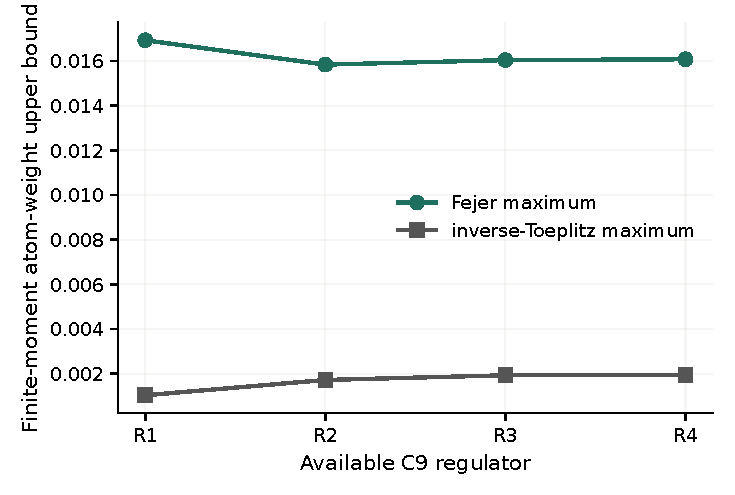
\includegraphics[width=.76\linewidth]{figures/spectral_atom_bounds.pdf}
\caption{Fej\'er and optimized inverse-Toeplitz bounds from thirteen stationary C9 moments. Both concern the same six source channels on finite regulators.}\label{fig:fejer-qict}
\end{figure}

For the full $13\times13$ block Toeplitz matrices, all four input sets are numerically positive definite. Their inverse-Toeplitz atom bounds are

\begin{table}[ht]
\centering\small
\caption{Optimized matrix-polynomial upper bounds $B_{13}(0)$, evaluated from the same thirteen stationary C9 moments. The improvement is relative to the Fej\'er maximum eigenvalue and carries the same finite-source interpretation.}\label{tab:christoffel-qict}
\begin{tabular}{@{}lrrr@{}}\toprule
Regulator & $\lambda_{\min}(B_{13})$ & $\lambda_{\max}(B_{13})$ & Fej\'er / optimized ratio\\\midrule
R1 & 0.0000507384 & 0.0010364794 & 16.34\\
R2 & 0.0000770880 & 0.0017207756 & 9.21\\
R3 & 0.0000773188 & 0.0019325137 & 8.30\\
R4 & 0.0000773178 & 0.0019562730 & 8.22\\
\bottomrule\end{tabular}
\end{table}

At R4, every eigenvalue of the zero-phase atomic weight is bounded by $0.0019562731$ in the nominal floating-point calculation, compared with the Fej\'er bound $0.0160835595$. The stored results include each $13$-block linear-solve residual and smallest Toeplitz eigenvalue. The $5\times5$ block tests give minimum eigenvalues approximately $2.68\times10^{-4}$, $4.78\times10^{-4}$, $5.03\times10^{-4}$ and $5.05\times10^{-4}$ for R1--R4. These are properties of the supplied six C9 matter-source channels. A transverse-traceless metric source defines a distinct spectral measure, to which the same mathematical bounds apply with its own moments and physical normalization.


\subsection{Finite identification, source visibility and the cyclic domain}
The truncated-moment example in Proposition~\ref{prop:indeterminate} establishes non-uniqueness for a class of admissible data. Particular finite moment sequences can identify a spectrum exactly. The appropriate distinction is between generic positive moment information and additional rank or invariance information.
\begin{proposition}[An exactly identifiable finite case]\label{prop:unitary-first-moment}
Let $W$ be unitary, $V^\dagger V=I_d$, and $C_1=V^\dagger WV$. If $C_1$ is unitary, then $WV=VC_1$, the source range reduces $W$, and $C_n=C_1^n$ for every integer $n$. Its source spectral measure is exactly the spectral measure of $C_1$.
\end{proposition}
\begin{proof}
The orthogonal component satisfies
\[
[(I-VV^\dagger)WV]^\dagger[(I-VV^\dagger)WV]=I-C_1^\dagger C_1=0.
\]
Thus $WV=VC_1$. Unitarity of $C_1$ makes the finite source range invariant under both $W$ and $W^\dagger$, giving the assertion by iteration. For example, $C_1=I_d$ fixes the source measure to $I_d\delta_1$.
\end{proof}
More generally, all source moments determine the unitary dynamics on the reducing cyclic subspace
\[
\mathcal K=\overline{\operatorname{span}}\{W^nVu:n\in\mathbb Z,\ u\in\mathbb C^d\}.
\]
Indeed, the moments determine every inner product between the displayed generating vectors. Two realizations with the same moments therefore have an isometric identification of their dense cyclic spans, extending to a unitary intertwiner on $\mathcal K$. Dynamics on $\mathcal K^\perp$ remain independent of the recorded source data. Proposition~\ref{prop:odd-nonidentification} is the parity-resolved instance of this source-visibility statement. Physical particle identification additionally specifies the energy branch, momentum dispersion and continuum state.

\subsection{Finite reconstruction from a stable moment rank}
\label{sec:flat-reconstruction}
The unitary-first-moment criterion extends to a source space generated by several transfer steps. In this setting, a stable Gram rank gives a finite reconstruction of the entire visible dynamics.
\begin{proposition}[Flat-rank reconstruction]\label{prop:flat-rank}
Let $C_0=I_d$ and suppose that the positive block Toeplitz matrix $T_{N+1}$ satisfies
\[
\operatorname{rank}T_{N+1}=\operatorname{rank}T_N=r.
\]
Then every unitary realization of these moments has the same $r$-dimensional cyclic source dynamics up to unitary equivalence. Its source measure is a finite sum of at most $r$ atoms, and the recorded moments determine all subsequent moments.
\end{proposition}
\begin{proof}
In a unitary realization define $\mathcal K_N=\operatorname{span}\{W^{-j}Vu:0\leq j<N\}$. The Gram matrix of these vectors is $T_N$. Equality of the two ranks therefore gives $\mathcal K_{N+1}=\mathcal K_N$. In particular, $W^{-1}\mathcal K_N\subseteq\mathcal K_N$. The restriction of $W^{-1}$ is an isometry of a finite-dimensional space onto itself, so $\mathcal K_N$ reduces $W$ and equals the full cyclic source space.

For an explicit reconstruction, factor $T_N=S^\dagger S$ with $S$ of full row rank $r$. Write $S^+$ for its Moore--Penrose inverse and form
\[
H_N=[C_{j-k-1}]_{j,k=0}^{N-1},\qquad
U_-=(S^+)^\dagger H_NS^+,\qquad Q=S_{[:,1:d]}.
\]
The columns of $S$ are coordinates of the source generators, while $H_N$ contains their inner products with the shifted generators. Thus $U_-$ represents $W^{-1}|_{\mathcal K_N}$ and is unitary. Every moment is
\begin{equation}\label{eq:flat-reconstruction}
C_n=Q^\dagger(U_-^\dagger)^nQ,\qquad n\in\mathbb Z.
\end{equation}
Diagonalization of $U_-^\dagger$ gives the phases and the positive matrix residues $Q^\dagger\Pi_jQ$, whose sum is $I_d$. A different full-row-rank Gram factor changes these coordinates by a unitary transformation and preserves the measure.
\end{proof}
For the normalized recorded C9 data, the exact positivity of $T_{13}$ gives $\operatorname{rank}T_{13}=78$, whereas $\operatorname{rank}T_{12}=72$. The supplied sequence therefore remains in the growing-rank regime. Its minimal cyclic realization has dimension at least 78. The independent reconstruction test uses a seven-dimensional unitary with two sources: $\operatorname{rank}T_4=\operatorname{rank}T_5=7$, and the recovered operator reproduces moments through order 21 to an operator-norm discrepancy below $2.5\times10^{-14}$. This test illustrates the exact rank criterion with explicitly declared finite matrices.

\subsection{Quantitative control near an invariant source space}
\begin{proposition}[Source-leakage bound]\label{prop:source-leakage}
Let $C_n=V^\dagger W^nV$, with $W$ unitary and $V$ a finite-dimensional isometry. Set $\varepsilon=\|I-C_1^\dagger C_1\|_2$. For every integer $n\geq1$,
\begin{equation}\label{eq:source-leakage}
\|C_n-C_1^n\|_2\leq\min\{2,\tfrac12n(n-1)\varepsilon\}.
\end{equation}
\end{proposition}
\begin{proof}
Write $P=VV^\dagger$. The two off-diagonal couplings obey
\[
\|(I-P)WV\|_2^2=\|I-C_1^\dagger C_1\|_2=\varepsilon,
\qquad \|V^\dagger W(I-P)\|_2^2=\|I-C_1C_1^\dagger\|_2=\varepsilon.
\]
The last equality follows from the common singular values of the square matrix $C_1$. Iterating the complementary-space equation gives $\|(I-P)W^kV\|_2\leq k\sqrt\varepsilon$, since both compressed blocks are contractions. Now
\[
C_{k+1}=C_1C_k+V^\dagger W(I-P)W^kV.
\]
Successive substitution bounds the difference from $C_1^n$ by $\sum_{k=1}^{n-1}k\varepsilon$. Both terms are contractions, which also gives the bound two.
\end{proof}
The estimate quantifies how accurately powers of the first moment represent the true moments over a finite transfer interval. Its exact zero-leakage case is Proposition~\ref{prop:unitary-first-moment}.

\subsection{Optimality and monotonicity of the Toeplitz bound}
The optimized bound is a matrix counterpart of the classical Christoffel extremal problem \cite{Simon05}. The following argument establishes its exact truncated-moment characterization directly.
\begin{proposition}[Feasible atomic weights and nested information]\label{prop:sharp}
Suppose $T_N\succ0$ and let $A=A_N(\theta)$. A positive component $M\delta_{e^{i\theta}}$ can be included in a positive matrix measure with the recorded moments if and only if
\[
T_N-AMA^\dagger\succeq0.
\]
The largest feasible component is the exact atomic weight $B_N(\theta)$ in an extremal representing measure, and, for compatible strictly positive successive moment matrices,
\begin{equation}\label{eq:nested-bounds}
0\preceq M_\theta\preceq B_{N+1}(\theta)\preceq B_N(\theta)\preceq F_N(\theta).
\end{equation}
\end{proposition}
\begin{proof}
Subtracting the proposed atom leaves the block Toeplitz matrix of the residual moments. A positive block Toeplitz matrix admits a positive matrix-valued representing measure: factor its Gram form, identify the shift between equal-length overlapping polynomial spans, and extend that isometry to a unitary after an auxiliary-space completion. Its spectral resolution supplies the residual measure. Adding the proposed atom recovers the original moments. Necessity follows directly by integrating its positive contribution.

For the maximal bound define $L_*=T_N^{-1}A(A^\dagger T_N^{-1}A)^{-1}$. It satisfies $A^\dagger L_*=I_d$. Every other $L$ satisfying this constraint can be written $L=L_*+Q$, $A^\dagger Q=0$, whence
\[
L^\dagger T_NL=B_N+Q^\dagger T_NQ\succeq B_N.
\]
Equivalently, $T_N-AB_NA^\dagger\succeq0$, and $AMA^\dagger\preceq T_N$ implies $M\preceq B_N$ by multiplication with $L_*^\dagger,L_*$. At this maximum the residual measure has zero additional atom at $e^{i\theta}$, since any positive additional weight would violate the upper bound. Increasing $N$ restricts the feasible set; alternatively, append a zero coefficient to any lower-degree polynomial. This proves monotonicity. The uniform polynomial gives $F_N$.
\end{proof}
For singular $T_N$, direct inversion is replaced by the exact conditions
\[
\operatorname{ran}(AM^{1/2})\subseteq\operatorname{ran}T_N,
\qquad M^{1/2}A^\dagger T_N^+AM^{1/2}\preceq I_d,
\]
where $T_N^+$ is the Moore--Penrose inverse. These follow by factoring through $T_N^{1/2}$ on its range. They cover finitely identifiable singular cases without applying a positive-definite inverse outside its domain.

\subsection{Finite-resolution spectral weight and controlled moment errors}
For $N\geq2$, let $I_{\theta,\delta}$ be the circular arc within distance $\delta$ of $\theta$, with $0<\delta<\pi/(N-1)$. Centering the phases in the Fej\'er polynomial gives
\[
\left|\frac1N\sum_{j=0}^{N-1}e^{ijt}\right|^2
\geq\cos^2\!\left(\frac{(N-1)\delta}{2}\right)=:a_{N,\delta}>0
\quad (|t|\leq\delta).
\]
Each centered cosine is at least $\cos((N-1)\delta/2)$; summing proves the inequality. Positivity then yields the finite-resolution bound
\begin{equation}\label{eq:arc-bound}
0\preceq\mu(I_{\theta,\delta})\preceq a_{N,\delta}^{-1}F_N(\theta).
\end{equation}
Equation~\eqref{eq:arc-bound} constrains the total weight of an unresolved narrow feature. Its positive lower enclosures are given by additional support hypotheses, as in Proposition~\ref{prop:exponential-gap}.

For verified moment errors $\|C_k-\widehat C_k\|\leq\delta_k$, a more flexible certificate uses fixed polynomial coefficients $L_j$ satisfying $\sum_j e^{-ij\theta}L_j=I_d$. Its exact quadratic form and error budget are
\begin{equation}\label{eq:polynomial-error}
M_\theta\preceq L^\dagger T_N L
\preceq L^\dagger\widehat T_NL+\mathcal E_LI_d,\qquad
\mathcal E_L=\sum_{j,k=0}^{N-1}\delta_{|j-k|}\|L_j\|\|L_k\|.
\end{equation}
The first inequality follows from $T_N\succeq AM_\theta A^\dagger$; the second follows term by term from the operator norm inequality. Unlike an inverse perturbation estimate, this certificate can be checked using a proposed polynomial without certifying a numerical inverse.

\subsection{An exact rational certificate for the recorded C9 data}
All supplied $6\times6$ moments are diagonal, with three identical left-source entries and three identical right-source entries. We retain every input array unchanged and define a precisely normalized recorded moment problem by
\[
\widetilde C_0=I_6,\qquad
\widetilde C_k=S^{-1/2}C_kS^{-1/2}\ (k\geq1),\qquad
S=\operatorname{Re}C_0.
\]
The maximum normalization change in the input is of order $2.5\times10^{-14}$. The rational implementation interprets each stored binary number exactly, removes the tiny imaginary diagonal of $C_0$, and divides each scalar diagonal sequence by its positive real zeroth moment. It proves positivity by exact $13$-step $LDL^\dagger$ factorization in each of the eight distinct scalar blocks. A numerical solve proposes coefficients; exact rational arithmetic enforces their sum to one and evaluates their polynomial energy. The final outward-rounded upper bounds are

\begin{table}[htbp]\centering\small
\caption{Exact-rational polynomial bounds for the explicitly normalized recorded finite moment problem. Independent physical moment and continuum errors enter through Eq.~\eqref{eq:polynomial-error}.}
\begin{tabular}{@{}lrr@{}}\toprule
Regulator & Left-source upper weight & Right-source upper weight\\\midrule
R1 & 0.001036479358 & 0.000050738373\\
R2 & 0.001720775586 & 0.000077087987\\
R3 & 0.001932513690 & 0.000077318759\\
R4 & 0.001956273015 & 0.000077317777\\
\bottomrule
\end{tabular}\label{tab:exact-rational}
\end{table}

The polynomial certificate is exact for this finite recorded-data problem. The full interacting QICT source family and its regulator limit retain their separate physical error budget. This distinction makes the arithmetic guarantee explicit while preserving the physical interpretation of the six matter-source channels.

\subsection{Convergence of the optimal atomic-weight hierarchy}
\begin{proposition}[Recovery of a source-visible atom]\label{prop:atom-limit}
For one fixed normalized matrix spectral measure with strictly positive $T_N$ at every order,
\[
B_N(\theta)\downarrow\mu(\{e^{i\theta}\})\quad\text{as }N\to\infty.
\]
If all remaining support is separated by an angular gap $\Delta$, then
\[
0\preceq B_N(\theta)-M_\theta\preceq q_N(I_d-M_\theta),
\qquad q_N=\min\{1,[N^2\sin^2(\Delta/2)]^{-1}\}.
\]
\end{proposition}
\begin{proof}
The normalized Fej\'er integrand tends pointwise to one at the specified phase and to zero at every other phase, and is bounded by one. Dominated convergence for the finite positive trace measure gives $F_N\to M_\theta$ in the finite source dimension. The inequalities $M_\theta\preceq B_N\preceq F_N$, together with monotonicity, prove the first claim. The gap estimate in Proposition~\ref{prop:fejer} gives the stated quantitative squeeze.
\end{proof}
This limit concerns a fixed measure. The uniform-gap statement below gives an explicit sufficient condition for a joint regulator and moment limit.

\subsection{Exponential bounds under a certified angular gap}
\label{sec:gap-filter}
An angular gap permits a sharper polynomial filter than the uniform Fej\'er average. Let $0<\Delta<\pi$, $c_\Delta=\cos(\Delta/2)$ and $m=N-1\geq1$. Denote the Chebyshev polynomial of the first kind by $\mathsf T_m$. Define ordinary polynomials by
\[
P_0(z)=1,\quad P_1(z)=\frac{1+z}{2c_\Delta},\quad
P_{m+1}(z)=\frac{1+z}{c_\Delta}P_m(z)-zP_{m-1}(z),
\qquad p_m(z)=\frac{P_m(z)}{\mathsf T_m(c_\Delta^{-1})}.
\]
The recurrence gives $p_m(1)=1$. For a specified phase $\theta$, set
\[
Q_{m,\Delta}(\theta)=\int|p_m(e^{i(\varphi-\theta)})|^2\,\dd\mu(\varphi),
\qquad
q_{m,\Delta}=\operatorname{sech}^2\!\left[m\operatorname{arcosh}(c_\Delta^{-1})\right].
\]
The quadratic form $Q_{m,\Delta}$ uses only $C_0,\ldots,C_m$.
\begin{proposition}[Exponential enclosure of an isolated atom]\label{prop:exponential-gap}
If the support outside $e^{i\theta}$ lies at circular distance at least $\Delta$, then
\begin{equation}\label{eq:exponential-gap}
\frac{Q_{m,\Delta}-q_{m,\Delta}I_d}{1-q_{m,\Delta}}
\preceq M_\theta\preceq B_{m+1}(\theta)\preceq Q_{m,\Delta},
\end{equation}
where $B_{m+1}$ is defined when $T_{m+1}\succ0$. In particular,
\begin{equation}\label{eq:exponential-convergence}
0\preceq B_{m+1}(\theta)-M_\theta
\preceq q_{m,\Delta}(I_d-M_\theta),\qquad
q_{m,\Delta}\leq4e^{-2m\operatorname{arcosh}(c_\Delta^{-1})}.
\end{equation}
\end{proposition}
\begin{proof}
On the unit circle the recurrence gives
\[
P_m(e^{it})=e^{imt/2}\mathsf T_m\!\left(\frac{\cos(t/2)}{c_\Delta}\right).
\]
For $\Delta\leq|t|\leq\pi$, the argument lies in $[0,1]$, where $|\mathsf T_m|\leq1$. At $t=0$, the normalized modulus equals one. Over the intervening arc it is at most one because $\mathsf T_m(x)=\cosh(m\operatorname{arcosh}x)$ is increasing for $x\geq1$. Consequently
\[
M_\theta\preceq Q_{m,\Delta}\preceq M_\theta+q_{m,\Delta}(I_d-M_\theta).
\]
The polynomial extremal characterization gives $B_{m+1}\preceq Q_{m,\Delta}$. Rearrangement and $\cosh x\geq e^x/2$ establish both claims.
\end{proof}
For a known gap $\Delta=0.55$ and thirteen moments, the exponential remainder factor is $0.00498661$, compared with $0.0802460$ for the uniform-polynomial gap bound. These numbers refer to the stated gap hypothesis. The C9 upper bounds in Tables~\ref{tab:fejer-qict}--\ref{tab:exact-rational} retain their direct finite-moment interpretation.

The same estimate controls a simultaneous regulator limit. Suppose normalized measures $\mu_{\mathcal R}$ converge weakly to $\mu$, all have the same fixed phase and excluded punctured arc of width $\Delta$, and their moment matrices at the required orders are positive definite. A continuous function equal to one at $\theta$ and zero outside that arc gives $M_{\theta,\mathcal R}\to M_\theta$. Equation~\eqref{eq:exponential-convergence} then yields
\[
\|B_{N,\mathcal R}(\theta)-M_\theta\|_2
\leq q_{N-1,\Delta}+\|M_{\theta,\mathcal R}-M_\theta\|_2.
\]
Thus both orders of the regulator and moment limits recover the same atom under the stated uniform gap and weak-convergence assumptions. Verified moment errors are added through Eq.~\eqref{eq:polynomial-error}.

\section{Operator reconstruction and certified finite spectra}
\label{sec:operator-spectrum}
The supplied C9 archive contains the neutral and charged transfer matrices, the weak source and the primitive vectors used to construct the recorded moments. These additional data specify a finite operator problem. We first recover the moment construction, including coherences within joint neutral eigenspaces, and then establish a spectral separation certificate that holds for every stationary state of the defined finite unitary model.

\subsection{The stationary finite Lehmann measure}
\label{sec:finite-lehmann}
Let $U_0=\sum_a z_aP_a$ and $U_f=\sum_b w_bQ_b$ be finite unitaries, let $S$ be an isometric source, and let $\rho\succeq0$ have unit trace and commute with $U_0$. The neutral spectral projectors include each complete degenerate eigenspace. The relative physical moments are
\[
C_n=\operatorname{Tr}\!\left(\rho U_0^{-n}S^\dagger U_f^nS\right).
\]
\begin{proposition}[Finite stationary spectral reconstruction]\label{prop:finite-lehmann}
For every integer $n$, the moments and their source resolvent have the representations
\begin{align}
C_n&=\sum_{a,b}p_{ba}(w_b\overline z_a)^n,
&p_{ba}&=\bigl\|Q_bSP_a\sqrt\rho\bigr\|_{\mathrm F}^2,\label{eq:finite-lehmann}\\
G(\zeta)&=\sum_{a,b}\frac{p_{ba}}{\zeta-w_b\overline z_a},
&p_{ba}&\geq0,\qquad\sum_{a,b}p_{ba}=1.\label{eq:finite-resolvent}
\end{align}
Consequently, the exact weight at phase zero is the sum of $p_{ba}$ over pairs with $w_b=z_a$.
\end{proposition}
\begin{proof}
Stationarity makes $\rho$ block diagonal in the projectors $P_a$. Insert both spectral decompositions in $C_n$ and use cyclicity of the trace. The coefficient of $(w_b\overline z_a)^n$ is
$\operatorname{Tr}(\rho P_aS^\dagger Q_bSP_a)$, equal to the displayed squared Frobenius norm. Summing the projectors and using $S^\dagger S=I$ gives normalization. The spectral theorem then gives Eq.~\eqref{eq:finite-resolvent}, and the term at relative eigenvalue one has precisely the stated weight.
\end{proof}
For several sources, the same construction replaces $p_{ba}$ by their positive Gram matrix. The recorded six-source problem consists of three identical left-source entries and three identical right-source entries.

For a primitive vector $v$, the stationary selection is
\[
\rho=\sum_aP_a|v\rangle\langle v|P_a.
\]
This expression retains all coherences within a degenerate joint eigenspace. In a numerical eigenbasis, write $v=\sum_i c_i|i\rangle$ and let $\mathcal G$ denote the chosen joint clusters. Comparing the corresponding coherent and diagonal densities gives the useful bound
\begin{equation}\label{eq:coherence-error}
\|\rho_{\mathcal G}-\rho_{\rm diag}\|_1
\leq\sum_{g\in\mathcal G}\sum_{\substack{i,j\in g\\i\ne j}}|c_i c_j|
=:\varepsilon_{\rm coh}.
\end{equation}
Each matrix unit $|i\rangle\langle j|$ has trace norm one, so the triangle inequality proves the result. For every contraction $B$, trace duality gives
$|\operatorname{Tr}[(\rho_{\mathcal G}-\rho_{\rm diag})B]|\leq\varepsilon_{\rm coh}$. In particular, this controls every unitary-source moment, uniformly in its order, when the operator family and basis are held fixed.

The numerical reconstruction retains the joint clusters of the original prescription, with chord tolerance $10^{-12}$. It reproduces all thirteen recorded moments at all four regulators with maximum entry discrepancy $2.68\times10^{-14}$. For the stored cluster coordinates, the right-hand side of Eq.~\eqref{eq:coherence-error} is zero at R1 and R2, $1.543\times10^{-14}$ at R3, and $1.052\times10^{-14}$ at R4. These are floating-point evaluations of the stated construction. The certificate below uses the operators directly and holds independently of this numerical clustering choice.

\subsection{A verified unitary interpretation of the stored matrices}
\label{sec:operator-disks}
An array stored in binary arithmetic defines an exact matrix $A$. We fix its unitary representative by the polar factor \cite{Higham86}
\begin{equation}\label{eq:polar-model}
U=A(A^\dagger A)^{-1/2}.
\end{equation}
The rectangular weak source is normalized by the corresponding map $S=A_S(A_S^\dagger A_S)^{-1/2}$. Positive lower singular-value bounds make both definitions unique. Across all twenty square input matrices, the certified distance satisfies $\|U-A\|_2\leq8.724\times10^{-14}$. Thus the operator statement refers to a precisely defined finite model, with an explicit distance to its stored numerical arrays.

\begin{proposition}[Residual certificate for polar-unitary spectra]\label{prop:polar-disks}
Let $Q$ be a square approximate eigenbasis and $D=\operatorname{diag}(d_j)$. Suppose verified upper bounds satisfy
\[
\|A^\dagger A-I\|_2\leq\delta_A<\tfrac12,\qquad
\|Q^\dagger Q-I\|_2\leq\delta_Q<\tfrac12,\qquad
\|AQ-QD\|_2\leq r.
\]
Every eigenvalue of the unitary in Eq.~\eqref{eq:polar-model} lies within distance
\begin{equation}\label{eq:polar-disk-radius}
\varepsilon=(1+\delta_Q)\bigl[r+\delta_A(1+\delta_Q)\bigr]
\end{equation}
of at least one centre $d_j$.
\end{proposition}
\begin{proof}
The singular values of $A$ give $\|U-A\|_2\leq\delta_A$, since
$|\sigma-1|=|\sigma^2-1|/(\sigma+1)\leq\delta_A$.
The singular values of $Q$ imply
$\|Q\|_2\leq1+\delta_Q$ and $\|Q^{-1}\|_2\leq1+\delta_Q$ for $0\leq\delta_Q<1/2$. Hence
\[
Q^{-1}UQ=D+E,\qquad
\|E\|_2\leq(1+\delta_Q)\bigl[r+\delta_A(1+\delta_Q)\bigr].
\]
If a point is farther than $\|E\|_2$ from every diagonal entry of $D$, then the Neumann series for $I-(\zeta-D)^{-1}E$ proves that $\zeta-D-E$ is invertible. Every eigenvalue therefore belongs to the union of the stated disks.
\end{proof}

The implementation obtains candidate centres and bases by a complex Schur decomposition. It then encloses each elementary real operation by outward rounding to the adjacent binary64 values. Complex matrix products are evaluated entry by entry through interval operations. For any residual $R$, the resulting bounds use
$\|R\|_2\leq\max\{\|R\|_1,\|R\|_\infty\}$; interval sums enclose both norms. The spectral guarantee thus depends on the verified residuals, independently of the eigensolver's accuracy estimate. Separate exact-rational checks cover the interval matrix products, including cancellation and subnormal arithmetic.

\subsection{Certified separation of the zero-phase component}
\label{sec:zero-phase-certificate}
Write the five polar unitaries as $U_{Y0},U_{YL},U_{YR},U_{W0},U_{WL}$, corresponding to the stored neutral, left and right $U(1)$ matrices and the neutral and charged $SU(2)$ matrices. Their finite tensor structure is
\[
U_0=U_{Y0}\otimes U_{W0},\quad
U_L=U_{YL}\otimes U_{WL},\quad
U_R=U_{YR}\otimes U_{W0},\qquad
S_L=I\otimes S,\quad S_R=I.
\]
The left relative phases are products of four factor eigenvalues. In the right physical trace, the common $SU(2)$ factor cancels:
\[
C_n^R=\operatorname{Tr}\!\left[\rho_Y U_{Y0}^{-n}U_{YR}^n\right],
\qquad \rho_Y=\operatorname{Tr}_{W}\rho.
\]
Joint stationarity implies $[\rho_Y,U_{Y0}]=0$, by taking the partial trace of $U_0\rho U_0^\dagger=\rho$. The source-visible right phases therefore depend on two $U(1)$ eigenvalues.

To combine the disks, let $k=2$ or $4$, let $p$ be a product of their centres, and suppose each centre has modulus less than two. Telescoping the product, using unit modulus for the exact eigenvalues, bounds its error by $2^{k-1}\sum_j\varepsilon_j$. If an outward-rounded calculation gives a common lower bound $d_*$ on $|p-1|$ for every candidate combination, then
\begin{equation}\label{eq:certified-chord-gap}
|z-1|\geq g:=d_*-2^{k-1}\sum_j\varepsilon_j
\end{equation}
for every relevant exact relative eigenvalue. The code bounds $|p-1|$ below by $\max\{|\operatorname{Re}p-1|,|\operatorname{Im}p|\}$ with interval endpoints; every candidate is included, even when its source weight vanishes.

\begin{table}[htbp]\centering\small
\caption{Certified chord-distance lower bounds for the polar-unitary finite C9 model. Displayed positive bounds are rounded down. The left column of candidate counts includes the entire relative tensor spectrum; the right source uses the exact spectator cancellation.}\label{tab:operator-gaps}
\begin{tabular}{@{}lrrrr@{}}\toprule
Regulator & Left candidates & $g_L$ & Right candidates & $g_R$\\\midrule
R1 & 4050 & $4.95900\times10^{-4}$ & 81 & $7.93216\times10^{-3}$\\
R2 & 306250 & $6.03108\times10^{-6}$ & 625 & $3.38493\times10^{-3}$\\
R3 & 6050520 & $2.43022\times10^{-8}$ & 2401 & $2.41273\times10^{-3}$\\
R4 & 59541075 & $1.92308\times10^{-7}$ & 6561 & $3.19912\times10^{-4}$\\
\bottomrule\end{tabular}
\end{table}

\begin{proposition}[Zero-phase weight in the finite C9 operator model]\label{prop:finite-zero-weight}
For each of the four polar-unitary models specified above, every stationary density gives
\begin{equation}\label{eq:finite-zero-weight}
\mu_L(\{1\})=\mu_R(\{1\})=0.
\end{equation}
The result holds for all three copies of each source. For either normalized source measure, its certified gap $g$ also gives
\begin{equation}\label{eq:finite-long-time}
F_N(0)\leq\min\!\left\{1,\frac{4}{N^2g^2}\right\},\qquad
|G(1)|\leq g^{-1}.
\end{equation}
\end{proposition}
\begin{proof}
The strictly positive verified bounds in Table~\ref{tab:operator-gaps} separate every left relative eigenvalue and every source-visible right relative eigenvalue from one. Equation~\eqref{eq:finite-lehmann} then places the entire positive measure at separated phases. For such a phase,
\[
\left|\frac1N\sum_{j=0}^{N-1}z^j\right|
=\left|\frac{1-z^N}{N(1-z)}\right|\leq\min\{1,2/(Ng)\}.
\]
Integrating its square proves the Fej\'er estimate. The resolvent bound follows by integrating $|1-z|^{-1}\leq g^{-1}$ against the normalized measure.
\end{proof}

This certificate uses more information than the truncated moment problem. The positive upper weights in Tables~\ref{tab:fejer-qict}--\ref{tab:exact-rational} describe all measures compatible with thirteen recorded moments. Equation~\eqref{eq:finite-zero-weight} selects the additional conclusion supplied by the finite operator model. The arrays and their normalized recorded-data certificate remain byte-for-byte unchanged.

The separation is stable under controlled changes of the unitary factors. If their operator-norm errors are bounded by $\eta_j$, tensor-product telescoping bounds the relative-transfer change by $\sum_j\eta_j$. A total smaller than $g$ preserves separation from one by at least $g-\sum_j\eta_j$. For the right source, this statement preserves its common spectator factor and identity source. These bounds give an explicit admissible operator-error budget.

The four regulators are representation cutoffs of one linked two-face static component. A continuum conclusion is governed by a uniform gap and convergence of the same source family, as in Section~\ref{sec:gap-filter}. For example, $\mu_R=\delta_{e^{i/R}}$ has zero weight at one at every finite $R$, while its weak limit is $\delta_1$. This example specifies why the finite certificate and the joint-limit theorem have distinct hypotheses. Particle masses, odd-sector states and metric poles retain the physical source, branch and continuum prescriptions stated in the corresponding sections.

\section{Metric response and scale-independent gravitational matching}\label{sec:metric}
\subsection{The metric action and its normalization}

The gravitational and cosmological formulas use signature $(-,+,+,+)$ and the Einstein-action convention $c^3(R-2\Lambda)/(16\pi G)$. Under the two-derivative metric and diffeomorphism-Ward assumptions of the QICT construction, the effective action may be written
\begin{equation}
\Gamma_g=\int \dd^4x\sqrt{-g}\left(\frac{\hbar\gamma_R}{2\ell_*^2}R-\frac{\hbar\epsilon_0}{\ell_*^4}\right)+\Gamma_{\geq4}[g],\qquad \ell_*=c\tau_*.
\end{equation}
Here $\Gamma_{\geq4}$ collects local terms with four or more metric derivatives in the long-wavelength expansion; their source-normalized coefficients are separate from the displayed two-derivative action. Coefficient comparison gives the matching identities
\begin{equation}\label{eq:matching}
\boxed{G_{\rm QICT}=\frac{c^5\tau_*^2}{8\pi\hbar\gamma_R},\quad
\Lambda_{\rm QICT}=\frac{\epsilon_0}{\gamma_Rc^2\tau_*^2},\quad
u_{\Lambda,\rm QICT}=\frac{\hbar\epsilon_0}{c^3\tau_*^4}.}
\end{equation}
Here $u_\Lambda$ is an energy density and $x^0=ct$ in the action integral. The identities match the physically normalized metric coefficients $\gamma_R$ and $\epsilon_0$ to the dimensional gravitational quantities. The two coefficients refer to curvature and volume variations, respectively.

\begin{proposition}[Vacuum-energy non-identifiability from normalized matter moments]
Consider the set of normalized matter-sector transfer moments and connected matter correlators evaluated on one fixed background metric, without an absolute metric-response normalization. These data admit a family of effective actions with distinct coefficients multiplying $\int\dd^4x\sqrt{-g}$.
\end{proposition}
\begin{proof}
At the specified fixed metric, add a source-independent constant $\delta u\int\dd^4x\sqrt{-g}/c$ to the action. It multiplies the unnormalized partition function by a source-independent factor and therefore cancels from normalized expectation values and connected derivatives with respect to matter sources. In contrast, a metric variation of the added term changes the stress response by a contribution proportional to $\delta u\,g_{\mu\nu}$. Hence the matter correlator data leave $\delta u$ unidentifiable. Metric-source derivatives resolve this shift once their normalization and renormalization prescription are specified.
\end{proof}

\noindent The physical metric prediction is therefore a function of the common-state coefficients and their continuum error enclosure. On the positive-vacuum branch, their joint covariance propagates directly into the predicted cosmological constant.
A joint covariance matrix $\mathsf C$ of the microscopic coordinates $\bm p=(\ln\epsilon_0,\ln\gamma_R,\ln\tau_*)$, gives the first-order propagation law
\begin{equation}
\sigma_{\ln\Lambda}^2=\bm J_\Lambda\,\mathsf C\,\bm J_\Lambda^\top,
\qquad \bm J_\Lambda=(1,-1,-2).
\end{equation}
Its entries are common-state theoretical uncertainties. Observational posterior errors describe a separate covariance and enter only the reference-data comparison.

\subsection{A clock-independent vacuum target}

For $\gamma_R>0$, Eq.~\eqref{eq:matching} determines a clock-independent response ratio. Eliminating the receiver clock gives the exact identity
\begin{equation}\label{eq:operator-vacuum-invariant}
\boxed{\mathcal I_\Lambda:=\frac{\epsilon_0}{\gamma_R^2}
=\frac{8\pi\hbar G\Lambda}{c^3}=8\pi\Lambda\ell_P^2,\qquad
\ell_P^2:=\frac{\hbar G}{c^3}.}
\end{equation}
This is the dimensionless gravitational invariant already identified algebraically in the principal QICT article; its significance here is a \emph{numerical, clock-independent observational target}. Under the flat base-$\Lambda$CDM interpretation used by Planck, the published value $\Lambda\ell_P^2=(2.846\pm0.076)\times10^{-122}$ yields
\begin{equation}\label{eq:operator-vacuum-target}
\boxed{\mathcal I_{\Lambda,\mathrm{reference}}=(7.1528\pm0.1910)\times10^{-121}\quad(68\%\ \mathrm{reference\ uncertainty}).}
\end{equation}
This uncertainty describes the adopted Planck posterior. The rounded background point in Section~\ref{sec:structure} defines a separate nominal reference. Equation~\eqref{eq:operator-vacuum-target} applies to a spacetime-constant metric-volume term; dynamical dark-energy models instead use a time-dependent stress tensor \cite{Planck,DESI25}. The independently computed ratio and its common-state covariance define the corresponding theoretical comparison. On the branch $\gamma_R>0$, positive $\Lambda$ is equivalent to positive $\epsilon_0$.

\subsection{The constant-volume equation of state}
\label{sec:consistency}
For a spacetime-constant renormalized volume term, metric variation fixes the associated stress tensor and equation of state exactly.
\begin{proposition}[Constant volume term and the equation of state]\label{prop:w}
For $S_{\rm vac}=-\int\dd^4x\sqrt{-g}\,u_{\rm vac}/c$ in coordinates with $x^0=ct$, with $u_{\rm vac}$ independent of spacetime and of the metric, the associated stress tensor is $T_{\mu\nu}=-u_{\rm vac}g_{\mu\nu}$ and its pressure is $p=-u_{\rm vac}$. For $u_{\rm vac}\ne0$, its homogeneous perfect-fluid equation-of-state parameter is $w=-1$.
\end{proposition}
\begin{proof}
The metric variation is $\delta\sqrt{-g}=-\tfrac12\sqrt{-g}\,g_{\mu\nu}\delta g^{\mu\nu}$. Hence the volume term yields $T_{\mu\nu}= -u_{\rm vac}g_{\mu\nu}$ after restoring consistent stress-energy units. Comparing with the perfect-fluid tensor $T_{\mu\nu}=(u+p)U_\mu U_\nu/c^2+pg_{\mu\nu}$ gives $p=-u$ and thus $w=p/u=-1$ for nonzero $u$.\end{proof}

The implication fixes the equation of state conditional on the constant-volume action. Its magnitude is set by the separately normalized vacuum coefficient. A robust measured departure from $w=-1$ selects an extended dynamical stress sector; DESI DR2 provides data-combination-dependent tests of this possibility \cite{DESI25}.


\subsection{Finite source curvature and continuum metric coefficients}\label{sec:finite-gravity-rank}
The supplied nine-state matrix family supports a direct independent evaluation of its selected-state derivatives. Let $E_j,|j\rangle$ diagonalize $K_0$, with ground branch $j=0$, and let $K_q^\dagger=K_{-q}$. Define
\begin{align}
D(s)&=\sum_{j>0}\frac{\Delta_j\bigl(|\langle j|K_q|0\rangle|^2+|\langle j|K_{-q}|0\rangle|^2\bigr)}{s+\Delta_j^2},
\quad \Delta_j=E_j-E_0>0,\\
H_{q,-q}&=\langle0|K_{q,-q}^{(2)}|0\rangle-D(0).
\end{align}
The mixed derivative is the finite Lehmann--Kato energy curvature. Its connected spectral term and source-contact term are distinct observables. The input gap is $0.47$, and direct diagonalization gives
\begin{equation}\label{eq:finite-source-numbers}
\boxed{\begin{aligned}
D(0)&=0.1494933610746553,\\
\langle K_{q,-q}^{(2)}\rangle&=0.2003415648585009,\\
H_{q,-q}&=0.0508482037838456.
\end{aligned}}
\end{equation}
For $N_{\rm cell}=64$ at $q\ell_*=0.125$, the connected response per cell is $0.00233583376679$, whereas the energy curvature per cell is $0.000794503184123$. The latter quantity includes the contact term; it measures the stiffness of the selected source family.

The independent homogeneous source derivative is
\[
\frac{\langle K_{\rm vol}^{(1)}\rangle}{N_{\rm cell}}
=0.000235557962534.
\]
If its source coordinate $J$ is defined by $\partial_J\ln\sqrt{-g}=4$, division by that factor gives the source-volume representative $\epsilon_{0,\rm src}=5.88894906336\times10^{-5}$. The factor four specifies the metric-source convention of this representative. The input matrices by themselves supply the displayed derivatives, independently of a continuum metric interpretation.

A continuum curvature coefficient is the quadratic momentum coefficient of a physically normalized response. The nine-state family supplies the stated finite derivatives at $q\ell_*=0.125$. Their frequency dependence and the independent role of momentum and contact data are characterized by the following results.

\subsection{Analytic bounds on the finite connected response}
\label{sec:response-bounds}
The Lehmann weights in the nine-state calculation give more than the static susceptibility. Write
\[
w_j=|\langle j|K_q|0\rangle|^2+|\langle j|K_{-q}|0\rangle|^2,
\qquad a_n=\sum_{j>0}\frac{w_j}{\Delta_j^{2n+1}}.
\]
\begin{proposition}[Positive spectral response and controlled expansion]\label{prop:stieltjes-response}
For $s\geq0$ and every integer $n\geq0$,
\begin{equation}\label{eq:response-monotonicity}
(-1)^nD^{(n)}(s)=n!\sum_{j>0}\frac{w_j\Delta_j}{(s+\Delta_j^2)^{n+1}}\geq0.
\end{equation}
The Taylor series $D(s)=\sum_{n=0}^\infty(-s)^na_n$ converges for $|s|<\Delta_{\min}^2$. On the entire positive real axis its finite remainder satisfies
\begin{equation}\label{eq:response-remainder}
0\leq(-1)^{p+1}\left[D(s)-\sum_{n=0}^p(-s)^na_n\right]
\leq s^{p+1}a_{p+1}.
\end{equation}
\end{proposition}
\begin{proof}
Differentiate each positive rational summand. For the expansion, apply the exact geometric identity to $(1+s/\Delta_j^2)^{-1}$. The remainder in each term has sign $(-1)^{p+1}$ and magnitude
$w_j s^{p+1}/[\Delta_j^{2p+3}(1+s/\Delta_j^2)]$.
Summing proves the real-axis bound, while absolute convergence of the geometric series proves the analytic-disk statement.
\end{proof}
The supplied arrays give
\begin{equation}\label{eq:response-taylor-numbers}
\begin{aligned}
a_0&=0.1494933610746553,&a_1&=0.3536064776270250,\\
a_2&=1.296428153315946,&a_3&=5.532355252365083,
\end{aligned}
\qquad \Delta_{\min}^2=0.2209.
\end{equation}
All quantities are expressed in the dimensionless source units of the finite matrix family.

Useful global enclosures follow from the same weights. For $a_0>0$, let $\bar r=a_1/a_0$, $r_-=\Delta_{\max}^{-2}$ and $r_+=\Delta_{\min}^{-2}$. When $r_-<r_+$, define $\alpha=(\bar r-r_-)/(r_+-r_-)$. Convexity of $(1+sr)^{-1}$, first below by Jensen's inequality and then above by its endpoint chord, gives
\begin{equation}\label{eq:response-jensen}
\frac{a_0}{1+s\bar r}\leq D(s)\leq
a_0\left(\frac{1-\alpha}{1+sr_-}+\frac{\alpha}{1+sr_+}\right),\qquad s\geq0.
\end{equation}
For equal gaps, $r_-=r_+$ and the exact result is $D(s)=a_0/(1+sr_-)$; this treats the degenerate case directly. At $s=0.1$, the recorded family gives $0.12089684\leq D(0.1)=0.12326493\leq0.12489231$. The gap controls analyticity in frequency; a spatial momentum derivative belongs to the separately specified momentum-dependent source family.

\subsection{Independent contact and momentum information}
\label{sec:contact-independence}
The selected-state curvature can be characterized exactly at the level of source data. For a smooth real source family
\[
K(J)=K_0+JA+\tfrac12J^2B,
\]
with a nondegenerate ground state, differentiation of the eigenvalue equation gives
\begin{equation}\label{eq:source-curvature}
E_0''(0)=\langle0|B|0\rangle
-2\sum_{j>0}\frac{|\langle j|A|0\rangle|^2}{E_j-E_0}.
\end{equation}
Indeed, choose the derivative of the normalized eigenvector perpendicular to $|0\rangle$. Its excited-state components are $\langle j|0'\rangle=-\langle j|A|0\rangle/(E_j-E_0)$; substitution in the second derivative proves the formula. Replacing $B$ by $B+bI$ preserves $K_0$, $A$ and every connected two-source Lehmann weight, while shifting $E_0''(0)$ by $b$. This explicitly separates contact data from the connected response. Physical metric sources additionally obey their specified Ward identities and renormalization conditions.

Finite momentum samples likewise determine a function only within its declared functional class. For distinct positive samples $x_i=q_i^2$, an analytic response $h(x)$ and
\begin{equation}\label{eq:momentum-sample-family}
\widetilde h_\beta(x)=h(x)+\beta x\prod_{i=1}^m(x-x_i)
\end{equation}
have identical values at every $x_i$ and at zero, while
$\widetilde h_\beta'(0)=h'(0)+\beta\prod_i(-x_i)$.
If $h$ is strictly positive on a compact sampling interval, sufficiently small $|\beta|$ also preserves that positivity. Thus a finite list of values, even with a fixed volume term, allows distinct quadratic momentum coefficients. A specified derivative expansion with a remainder enclosure gives a precise alternative: for $h(x)=a+bx+R(x)$, $|R(x)|\leq Mx^2$,
\begin{equation}\label{eq:curvature-sample-bound}
\left|b-\frac{h(x)-a}{x}\right|\leq Mx\qquad(x>0).
\end{equation}
With verified errors $\delta_h$ and $\delta_a$, the right-hand side becomes $Mx+(\delta_h+\delta_a)/x$. These statements specify exactly how a curvature coefficient is identified from a physically normalized response.

\section{Particle interactions and thermal production}\label{sec:thermal}

\subsection{A neutral scalar and the scattering amplitude}\label{sec:scalar-scattering}
For a concrete collider and direct-detection test, let $S$ denote a stable real $Z_2$-odd scalar. This section specifies an additional effective particle model, with its own mass and coupling inputs. Particle amplitudes use signature $(+,-,-,-)$, $p^2=E^2-\mathbf p^2$, and $\hbar=c=1$ unless units are restored explicitly. This convention and the gravitational signature in Section~\ref{sec:metric} describe the same physical invariants after the corresponding metric-sign change. Consider
\begin{equation}
\mathcal L_S=\frac12(\partial_\mu S)^2-\frac12m_0^2S^2-\frac{\lambda_S}{4}S^4
-\frac{\lambda_{HS}}2S^2H^\dagger H,\qquad
m_S^2=m_0^2+\frac{\lambda_{HS}v^2}{2}.
\end{equation}
At low momentum transfer, Higgs exchange gives the leading tree-level spin-independent nucleon cross section
\begin{equation}\label{eq:si}
\sigma_{\rm SI}=\frac{\lambda_{HS}^2f_N^2\mu_{SN}^2m_N^2}{4\pi m_h^4m_S^2}
\times(\hbar c)^2,
\quad \mu_{SN}=\frac{m_Sm_N}{m_S+m_N},
\end{equation}
where particle masses and the first factor are expressed in natural units and the final factor converts to physical area. The scalar nucleon form factor $f_N$ carries a significant hadronic uncertainty and must be propagated in a physical fit. We use $m_h=125.1$ GeV, $m_N=0.939$ GeV, and $f_N=0.30$ solely as benchmark inputs.

For $m_S=40$ GeV and $\lambda_{HS}=0.01$, Eq.~\eqref{eq:si} yields
\begin{equation}
\boxed{\sigma_{\rm SI}(40\,\Gev)=5.282\times10^{-46}\ \mathrm{cm}^2.}
\end{equation}
The 2025 LUX--ZEPLIN combined-exposure result gives a 90\% confidence upper limit of $2.2\times10^{-48}\,\mathrm{cm}^2$ at $40$ GeV \cite{LZ25}. For comparison, the XENONnT 3.1 tonne-year analysis reports a 90\% minimum of $1.7\times10^{-47}\,\mathrm{cm}^2$ at $30$ GeV; the comparison at $40$ GeV uses the exclusion curve evaluated at that mass \cite{XENON25}. The 40-GeV illustrative point is about $240$ times the LZ limit at that mass and is excluded under the standard elastic nuclear-recoil assumptions. The exclusion concerns this selected effective-theory point and the assumed local scalar abundance. The published limit is a spin-independent elastic-scattering constraint for the adopted local-halo model \cite{LZ25}.

For the separate illustrative parameter choice $m_S=300$ GeV, $\lambda_{HS}=0.20$, Eq.~\eqref{eq:si} gives $3.910\times10^{-45}$ cm$^2$. Its experimental comparison is defined by the exclusion curve at $300$ GeV, the detector response and the local scalar fraction.

\subsection{The partial Higgs-pair contact rate}\label{sec:contact-rate}
The $S^2h^2$ contact vertex produces a partial annihilation rate
\begin{equation}
\left.\sigv\right|_{SS\to hh,\,\rm contact}
=\frac{\lambda_{HS}^2}{64\pi m_S^2}\sqrt{1-\frac{m_h^2}{m_S^2}},\qquad m_S>m_h.
\end{equation}
At $m_S=300$ GeV and $\lambda_{HS}=0.20$ this is $2.345\times10^{-26}$ cm$^3$ s$^{-1}$. Substitution into the frequently used thermal scaling $\Om_Sh^2\simeq0.12(2.2\times10^{-26}\,\mathrm{cm^3\,s^{-1}}/\sigv)$ gives $0.113$ \emph{for this partial-channel scaling estimate}. This partial-channel scaling isolates the contact contribution. The full tree-level two-body benchmark in Sec.~\ref{sec:portal-complete} includes interference, gauge and fermion final states, thresholds and thermal averaging. The abundance equation is
\begin{equation}
\frac{\dd Y}{\dd x}=-\frac{s(T)\sigv_{\rm full}(T)}{H(T)x}\bigl(Y^2-Y_{\rm eq}^2\bigr),\qquad x=m_S/T,
\end{equation}
for constant entropy degrees of freedom. With varying $g_{*s}$, entropy conservation supplies the factor $\mathcal A_s(T)$ derived below. The contact-only rate defines the limiting constant-rate equation below.

\subsection{Decay-driven freeze-in from an equilibrated parent}\label{sec:decay-freezein}
A distinct production model assumes a thermal scalar parent $A$ with mass $M_A$, one internal degree of freedom, and a feebly coupled stable daughter $S$. The parent undergoes $A\to S\varphi$, where $\varphi$ is a light bath particle, with partial width $\Gamma_A$. The exact parity assignment makes $A$ and $S$ odd and $\varphi$ even. The specified model takes $S$ to be the lightest odd particle and imposes $M_A>m_S+m_\varphi$; the allowed parent decay then preserves the daughter's parity protection. The model assumes bath interactions that equilibrate $A$ and a feeble daughter-production sector. For radiation domination, Maxwell--Boltzmann statistics, approximately constant entropy and energy degrees of freedom $g_{*s},g_{*\rho}$, and negligible inverse reactions,
\begin{align}
\gamma_{A\to S\varphi}&=\frac{g_A\Gamma_A M_A^2 T}{2\pi^2}K_1(M_A/T),\\
\frac{\dd Y_S}{\dd x}&=\frac{45g_A\Gamma_AM_{\rm Pl}}{4\pi^4\,1.66\,g_{*s}\sqrt{g_{*\rho}}\,M_A^2}
\,x^3K_1(x),\quad x=M_A/T.\label{eq:fimain}
\end{align}
The decay produces exactly one $S$ per event, so the source term and integrated yield have the normalization
\begin{equation}\label{eq:fi}
\boxed{Y_S(\infty)=\frac{135\,g_A\,\Gamma_AM_{\rm Pl}}
{8\pi^3\,1.66\,g_{*s}\sqrt{g_{*\rho}}\,M_A^2},}
\end{equation}
since $\int_0^\infty x^3K_1(x)\dd x=3\pi/2$. The number of dark particles per decay is fixed by the stated $A\to S\varphi$ channel. For a parent producing two $S$ particles, Eq.~\eqref{eq:fi} would acquire an additional factor of two. The equilibrium parent assumption specifies a bath-coupled parent whose thermalizing reactions are distinct from the feeble daughter-production channel.

Using $M_A=1000$ GeV, $m_S=10$ GeV, $g_{*s}=g_{*\rho}=106.75$, and a physical one-daughter decay width of $10^{-20}$ GeV gives
\begin{equation}
Y_S(\infty)=3.6292\times10^{-11},\qquad
\Om_Sh^2=2.742\times10^8\left(\frac{m_S}{\Gev}\right)Y_S
=\boxed{0.09951}.
\end{equation}
The rate-to-expansion ratio at $T=M_A$ is $\Gamma_A/H\simeq7.12\times10^{-9}$. This small ratio is a diagnostic of the specified feeble decay source. The calculation assumes that the stated decay dominates daughter production and that daughter thermalization is negligible. Adaptive quadrature of Eq.~\eqref{eq:fimain} from $x=10^{-3}$ gives the final-to-analytic ratio $0.9999999999293$, consistent with the finite-temperature estimate in Sec.~\ref{sec:finite-reheating}. The model uses constant $g_*$, instantaneous reheating, Maxwell--Boltzmann statistics and the single decay channel. Its masses and width are independent effective-model inputs. The limiting yield scales as $Y_\infty\propto \Gamma_A M_{\rm Pl}/(g_{*s}\sqrt{g_{*\rho}}M_A^2)$, so its logarithmic sensitivities are $\partial\ln Y/\partial\ln\Gamma_A=1$, $\partial\ln Y/\partial\ln M_A=-2$, $\partial\ln Y/\partial\ln g_{*s}=-1$, and $\partial\ln Y/\partial\ln g_{*\rho}=-1/2$. These derivatives propagate a specified parameter covariance into the yield covariance.

\begin{figure}[t]
\centering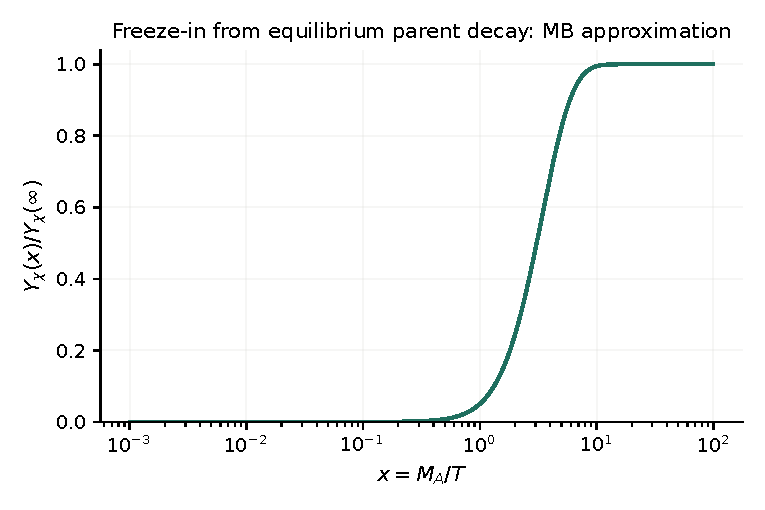
\includegraphics[width=.79\linewidth]{figures/freezein_yield.pdf}
\caption{Accumulated freeze-in yield in the explicit Maxwell--Boltzmann decay-source benchmark. The curve is normalized to its analytic asymptotic yield.}
\end{figure}

\subsection{Indirect-detection observables}
For the self-conjugate scalar $S$, annihilation produces a gamma-ray flux from a target with line-of-sight density factor $J$,
\begin{equation}
\frac{\dd\Phi_\gamma}{\dd E}=\frac{\sigv}{8\pi m_S^2}\frac{\dd N_\gamma}{\dd E}\,J,\qquad
J=\int_{\Delta\Om}\dd\Om\int \rho_S^2\,\dd\ell.
\end{equation}
For a specified final state, the Fermi--LAT likelihood combines the photon spectrum, branching fractions, density-squared $J$ factors and instrument response. The 14- and approximately 17-year dwarf-spheroidal analyses give bounds on the annihilation contribution \cite{Fermi24,Fermi26}. Antiproton inference additionally includes Galactic propagation, nuclear production and solar modulation \cite{AMS24}. These observables test the annihilation kernel of a specified candidate; the decay-only freeze-in example defines its production history through a separate collision term.

\subsection{Laboratory and abundance inversions}

For the selected scalar Higgs-portal normalization, the zero-momentum spin-independent cross section is quadratic in $\lambda_{HS}$, with other parameters held fixed. The original $m_S=40$ GeV, $\lambda_{HS}=0.01$ reference gives $\sigma^{\rm SI}_N=5.2815843\times10^{-46}$ cm$^2$. The LZ 4.2 tonne-year combined limit at this mass is $\sigma^{\rm SI}_{N,90}=2.2\times10^{-48}$ cm$^2$ \cite{LZ25}. Algebraic inversion, with the same halo model and nuclear conventions as the published limit, yields
\begin{equation}\label{eq:portalbound}
\boxed{|\lambda_{HS}|\leq 0.01\sqrt{\frac{2.2\times10^{-48}}{5.2815843\times10^{-46}}}=6.4540\times10^{-4}},\qquad
\frac{\sigma_N^{\rm SI}(0.01)}{\sigma_{N,90}^{\rm SI}}=240.07.
\end{equation}
This is a bound on the chosen low-energy portal model; its interpretation assumes that the candidate constitutes all of the local halo and scatters elastically and spin-independently. For a local fraction $0<f_{\rm loc}\leq1$ and the same velocity distribution, the rate constrains $f_{\rm loc}\sigma_{\rm SI}$ and the coupling bound scales as $f_{\rm loc}^{-1/2}$.  For a source-defined QICT candidate, the matched nucleon vertex supplies the amplitude in the same detector-response functional.

For one dark daughter per thermal parent decay, Eq.~\eqref{eq:fi} makes the asymptotic abundance linear in the partial decay width. Inverting the earlier reference scenario against the measured $\Omega_ch^2\simeq0.120$ \cite{Planck} yields
\begin{equation}\label{eq:widthinv}
\boxed{\Gamma_A^{\rm required}=1.205877\times10^{-20}\ \Gev,\qquad
\left.\frac{\Gamma_A}{H}\right|_{T=M_A}=8.58396\times10^{-9}.}
\end{equation}
Equation~\eqref{eq:widthinv} gives the decay width selected by the observed abundance within this effective production model.

\subsection{The constant-rate Boltzmann equation}
\label{sec:constant-freezeout}
A separate, specified freeze-out test evolves the comoving abundance with constant entropy/energy degrees of freedom, Maxwell--Boltzmann equilibrium and constant $s$-wave annihilation rate:
\begin{align}
\frac{\dd Y}{\dd x}&=-\frac{s\langle\sigma v\rangle}{Hx}(Y^2-Y_{\rm eq}^2),\qquad
Y_{\rm eq}=\frac{45g_\chi}{4\pi^4g_{*s}}x^2K_2(x),\\
\frac{s\langle\sigma v\rangle}{Hx}&=\frac{2\pi^2}{45\cdot1.66}\frac{g_{*s}}{\sqrt{g_{*\rho}}}\frac{M_{\rm Pl}m_\chi\langle\sigma v\rangle}{x^2}.
\end{align}
Numerical integration using $m_\chi=300$ GeV, $g_\chi=1$, $g_{*s}=g_{*\rho}=90$, and the previously stated contact-only reference rate $\langle\sigma v\rangle=2.345311\times10^{-26}$ cm$^3$s$^{-1}$, starting at $x=8$ in equilibrium, gives
\begin{equation}\label{eq:freezeoutfull}
\boxed{Y_\infty=1.219574\times10^{-12},\qquad
\Omega_\chi h^2=0.100322.}
\end{equation}
The integration uses a scaled abundance and an analytic late-time tail. An independent endpoint-and-step study is recorded in the numerical convergence data. This solves the specified constant-rate limiting Boltzmann equation. It is distinct from the thermally averaged portal calculation in Sec.~\ref{sec:portal-complete}, whose complete tree-level two-body amplitude supplies the physical annihilation rate within that benchmark.

\begin{figure}[t]\centering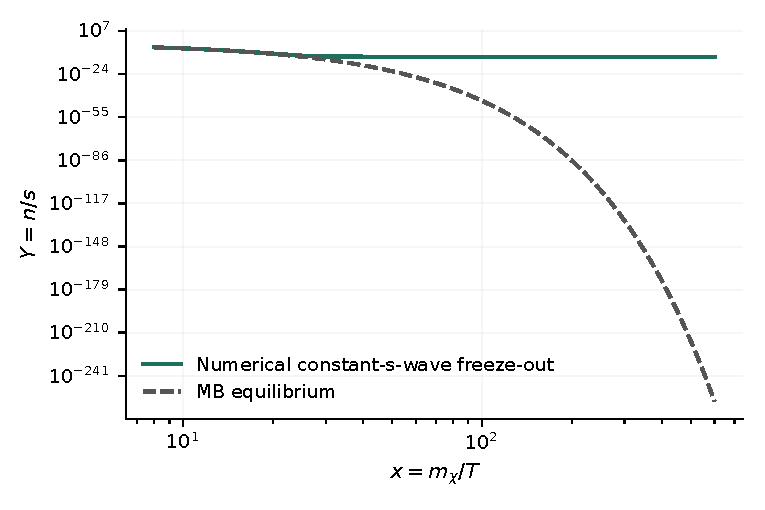
\includegraphics[width=.78\linewidth]{figures/freezeout_toy_exact_ode.pdf}\caption{Numerical solution of the fixed-rate single-species Boltzmann equation, with its Maxwell--Boltzmann equilibrium distribution. All masses and rates are external benchmark parameters.}\end{figure}

\subsection{Thermally averaged two-body Higgs-portal calculation}\label{sec:portal-complete}
The stated scalar interaction also determines a more complete, independently reproducible tree-level benchmark. With $\lambda=\lambda_{HS}$ and $v=246.22$ GeV, the Higgs-pair amplitude includes the contact, $s$-channel and both scalar-exchange diagrams:
\begin{equation}\label{eq:hh-amplitude}
\mathcal M_{hh}=-\lambda\left[1+\frac{3m_h^2}{s-m_h^2+im_h\Gamma_h}
+\lambda v^2\left(\frac1{t-m_S^2}+\frac1{u-m_S^2}\right)\right].
\end{equation}
The overall phase is immaterial. The symmetry factor for identical final Higgs particles gives
\begin{equation}
(\sigma v_{\rm M})_{hh}=\frac{\sqrt{1-4m_h^2/s}}{32\pi s}
\int_{-1}^{1}|\mathcal M_{hh}|^2\,\dd\cos\vartheta.
\end{equation}
Here $v_{\rm M}=2\sqrt{1-4m_S^2/s}$ in the centre-of-mass frame. Other open two-body channels are determined by the tree-level width of a virtual Higgs of invariant mass $\sqrt s$ \cite{Cline13}:
\begin{align}
(\sigma v_{\rm M})_{\rm SM\setminus hh}
&=\frac{2\lambda^2v^2\Gamma^{\rm tree}_{h\to WW,ZZ,f\bar f}(\sqrt s)}
{\sqrt s[(s-m_h^2)^2+m_h^2\Gamma_h^2]},\\
\Gamma_{f\bar f}(\sqrt s)&=\frac{N_c m_f^2\sqrt s}{8\pi v^2}
\left(1-\frac{4m_f^2}{s}\right)^{3/2},\\
\Gamma_{WW}(\sqrt s)&=\frac{s^{3/2}}{16\pi v^2}\sqrt{1-4r_W}
(1-4r_W+12r_W^2),\qquad r_V=m_V^2/s,
\end{align}
and $\Gamma_{ZZ}$ has the corresponding $1/(32\pi v^2)$ coefficient. Each contribution is included above its threshold. We use the vacuum input masses and fixed Yukawa representatives listed in the code; the propagator width is $\Gamma_h=4.07$ MeV. This defines a tree-level two-body benchmark with constant $g_{*s}=g_{*\rho}=90$. Quantum corrections, running couplings and thermal self-energies define additional physical refinements.

Maxwell--Boltzmann kinetic equilibrium gives the relativistic thermal average \cite{Gondolo91}
\begin{equation}\label{eq:thermal-average}
\langle\sigma v\rangle_T=\frac1{8m_S^4TK_2^2(m_S/T)}
\int_{4m_S^2}^{\infty}\sigma(s)(s-4m_S^2)\sqrt s\,K_1(\sqrt s/T)\,\dd s.
\end{equation}
Scaled Bessel functions and Gaussian quadrature evaluate this expression without exponential underflow. For the selected $m_S=300$ GeV, $\lambda=0.20$ point,
\begin{equation}\label{eq:portal-results}
\boxed{\begin{aligned}
(\sigma v)_{T\to0}&=1.13490\times10^{-25}\ \mathrm{cm^3\,s^{-1}},\\
\langle\sigma v\rangle_{x=20}&=9.78460\times10^{-26}\ \mathrm{cm^3\,s^{-1}},\\
Y_\infty&=2.85098\times10^{-13},\qquad \Omega_Sh^2=0.0234522.
\end{aligned}}
\end{equation}
The abundance is obtained by integrating the Boltzmann equation with the thermal rate and its post-endpoint annihilation tail. It is a conditional prediction of this specified Higgs-portal benchmark. The selected point supplies about $19.54\%$ of the reference $\Omega_ch^2=0.120$ through this thermal history; its direct-detection rate scales with the actual local scalar fraction. The contact-only calculation in Eq.~\eqref{eq:freezeoutfull} isolates a distinct limiting collision kernel.

\begin{figure}[htbp]\centering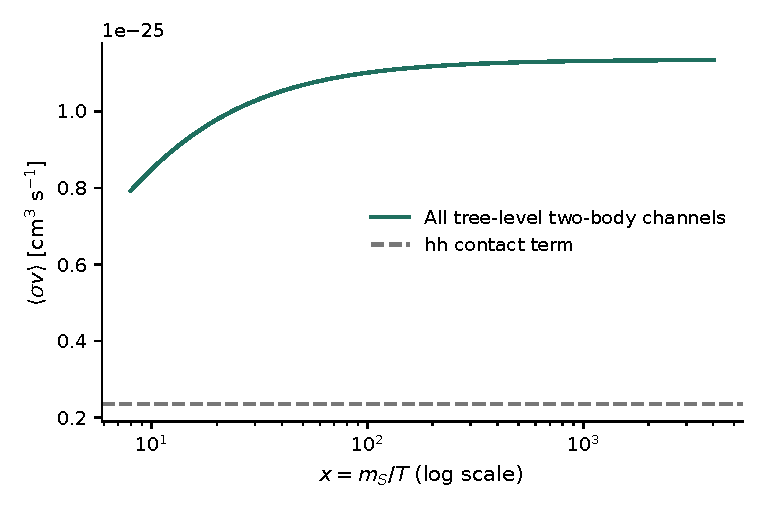
\includegraphics[width=.8\linewidth]{figures/portal_thermal_rates.pdf}
\caption{Thermally averaged annihilation into all tree-level two-body final states at the selected 300-GeV scalar point. The dashed line is the Higgs-pair contact contribution. Fixed vacuum parameters and constant relativistic degrees of freedom define the calculation.}\end{figure}

\subsection{The asymptotic tail of the constant-rate limiting equation}
For a constant annihilation coefficient $K$, the late equation is $Y'=-KY^2/x^2$ once $Y_{\rm eq}$ is exponentially small. Integration gives
\begin{equation}\label{eq:freezeout-tail}
\frac1{Y_\infty}=\frac1{Y(x_f)}+\frac K{x_f},\qquad
K=\frac{2\pi^2}{45\cdot1.66}\frac{g_{*s}}{\sqrt{g_{*\rho}}}M_{\rm Pl}m_\chi\langle\sigma v\rangle.
\end{equation}
For a temperature-dependent rate, replace $K/x_f$ by the corresponding integral over $\langle\sigma v\rangle(x)/x^2$. At $x_f=4000$, the constant-rate endpoint yield $1.2264721\times10^{-12}$ becomes $Y_\infty=1.2195738\times10^{-12}$, giving $\Omega_\chi h^2=0.10032214$. The tail contributes a $0.56245\%$ reduction relative to the endpoint abundance. At this endpoint the equilibrium correction is exponentially smaller than the stated numerical precision. The limiting equation assumes radiation domination and constant degrees of freedom throughout its formal late-time continuation.

\subsection{Finite reheating and a rigorous production-tail estimate}\label{sec:finite-reheating}
For instantaneous reheating to $T_{\rm RH}$ with zero initial daughter abundance, the one-daughter decay model has the exact limiting yield
\begin{equation}\label{eq:finite-reheating}
Y_\infty(T_{\rm RH})=Y_\infty(\infty)\,
\mathcal R(x_{\rm RH}),\qquad
\mathcal R(x)=\frac{2}{3\pi}\int_x^\infty t^3K_1(t)\,\dd t,
\quad x_{\rm RH}=M_A/T_{\rm RH}.
\end{equation}
The identity $(xK_1(x))'=-xK_0(x)<0$ and $xK_1(x)\to1$ imply $K_1(x)\leq1/x$. Therefore
\begin{equation}\label{eq:reheating-bound}
0\leq1-\mathcal R(x)\leq\min\{1,2x^3/(9\pi)\}.
\end{equation}
Direct quadrature gives $\mathcal R(0.1)=0.999929927$, $\mathcal R(1)=0.949556350$, and $\mathcal R(10)=0.005084288$. For the plotted history starting at $x=10^{-3}$, the omitted early production is bounded by $7.074\times10^{-11}$ of the high-temperature yield. The numerical-to-analytic ratio is $0.9999999999293$; this deficit is the stated finite starting temperature. The model assumes bath-maintained parent equilibrium and feeble daughter production \cite{Hall10}.

The leading freeze-out equation with temperature-dependent entropy degrees of freedom is also fixed by entropy conservation. Defining
\[
\mathcal A_s(T)=1+\frac13\frac{\dd\ln g_{*s}}{\dd\ln T},
\]
one obtains $\dot x=Hx/\mathcal A_s$ and
\[
\frac{\dd Y}{\dd x}=-\mathcal A_s\frac{s\langle\sigma v\rangle}{Hx}(Y^2-Y_{\rm eq}^2).
\]
The constant-degree examples set $\mathcal A_s=1$. The functions $g_{*s}(T)$, $g_{*\rho}(T)$ and the thermal collision kernel specify the temperature-dependent calculation.
\subsection{Clock cancellation in the decay yield}

The one-daughter, Maxwell--Boltzmann freeze-in calculation of Eq.~\eqref{eq:fi} admits an additional QICT-specific rewriting. In natural units $\hbar=c=k_B=1$, write the dimensional source quantities in common microscopic units,
\begin{equation}
M_A=\varepsilon_AE_*,\qquad\Gamma_A=\delta_AE_*,\qquad
E_*=\tau_*^{-1},\qquad M_{\mathrm{Pl}}=G^{-1/2}=\sqrt{8\pi\gamma_R}\,E_*.
\end{equation}
For an equilibrated parent with $g_A$ internal states, one dark daughter per decay, radiation domination and constant $g_{*s}$ and $g_{*\rho}$, the integrated collision term is
\begin{align}
Y_\chi(\infty)&=\frac{135g_A}{8\pi^3\,1.66\,g_{*s}\sqrt{g_{*\rho}}}\frac{\Gamma_A M_{\rm Pl}}{M_A^2}\\
&=\boxed{\frac{135g_A\sqrt{8\pi\gamma_R}}{8\pi^3\,1.66\,g_{*s}\sqrt{g_{*\rho}}}\frac{\delta_A}{\varepsilon_A^2}}.\label{eq:operator-fi-scale}
\end{align}
The receiver scale cancels exactly from the yield. In a common-state description, $\varepsilon_A$, $\delta_A$ and $\gamma_R$ are its dimensionless physical inputs, together with the equilibrium and production assumptions. The abundance conversion $\Omega_\chi h^2=2.742\times10^8(m_\chi/\mathrm{GeV})Y_\chi$ additionally uses the physical daughter mass and cosmological entropy normalization. The transformation has been checked at several common energy coordinates while holding $M_A$, $\Gamma_A$ and $M_{\rm Pl}$ fixed: both parameterizations give $Y_\chi=3.629199\times10^{-11}$ for the selected 1000-GeV parent model.


\subsection{A rigorous enclosure of residual equilibrium production}
\label{sec:thermal-tail-bound}
The late-time tail can be bounded while retaining the equilibrium source. Let $Y'=-\lambda(x)(Y^2-Y_{\rm eq}^2)$ on $x\geq x_f$, with $\lambda\geq0$, $Y(x_f)=Y_f>0$, and finite $\int_{x_f}^\infty\lambda\,\dd x$. Define
\begin{align}
Y_0(x)&=\left[Y_f^{-1}+\int_{x_f}^x\lambda(t)\,\dd t\right]^{-1},\\
I_0&=Y_f^{-1}+\int_{x_f}^\infty\lambda(x)\,\dd x,\qquad
E=\int_{x_f}^\infty\lambda(x)\left[\frac{Y_{\rm eq}(x)}{Y_0(x)}\right]^2\dd x.
\end{align}
\begin{proposition}[Positive-source tail enclosure]\label{prop:thermal-tail}
For a positive solution with finite $E<I_0$,
\begin{equation}\label{eq:thermal-tail-bracket}
\boxed{I_0^{-1}\leq Y_\infty\leq(I_0-E)^{-1}.}
\end{equation}
\end{proposition}
\begin{proof}
The reciprocal yield obeys $(1/Y)'=\lambda[1-(Y_{\rm eq}/Y)^2]\leq\lambda$. Integration gives $Y(x)\geq Y_0(x)$. A second integration yields
\[
0\leq I_0-Y_\infty^{-1}
=\int_{x_f}^\infty\lambda(Y_{\rm eq}/Y)^2\,\dd x\leq E.
\]
The finite integrals and $I_0-E>0$ ensure a positive finite limit; inversion proves the result.
\end{proof}
For the constant-rate example, starting this estimate already at $x_f=30$ gives a numerically evaluated relative interval width $4.07\times10^{-7}$. The corresponding endpoints are approximately $1.21957328\times10^{-12}$ and $1.21957378\times10^{-12}$ for the computed $Y_f$. An independent integration retaining the equilibrium source lies within this interval to numerical precision. The analytic inequalities are exact for fixed $Y_f$ and collision kernel; numerical initial-value and quadrature errors remain explicit parts of their evaluation.

\subsection{Temperature dependence and exact reheating sensitivity}
Entropy conservation gives the one-daughter decay yield for temperature-dependent degrees of freedom in a compact form. Set $x=M_A/T$, assume an equilibrated Maxwell--Boltzmann parent, radiation domination with $H=1.66\sqrt{g_{*\rho}}T^2/M_{\rm Pl}$, conserved entropy and $\mathcal A_s>0$. For zero initial daughter abundance,
\begin{equation}\label{eq:variable-g-freezein}
Y_\infty=\frac{45g_A\Gamma_AM_{\rm Pl}}{4\pi^4\,1.66\,M_A^2}
\int_{x_{\rm RH}}^\infty
\frac{\mathcal A_s(M_A/x)}{g_{*s}(M_A/x)\sqrt{g_{*\rho}(M_A/x)}}
x^3K_1(x)\,\dd x.
\end{equation}
This follows by dividing $\dot n_S+3Hn_S=\gamma_{A\to S\varphi}$ by the conserved entropy density and using $\dot x=Hx/\mathcal A_s$. For a constant width, the displayed formula is exact within those thermodynamic assumptions. A temperature-dependent partial width enters inside the integral. If the positive thermodynamic factor is bounded between $F_-$ and $F_+$ over the production range, multiplying the constant-kernel integral by these extrema gives a two-sided yield bound.

In the constant-degree model, differentiation with respect to the reheating temperature gives
\begin{equation}\label{eq:reheat-sensitivity}
\frac{\partial\ln Y_\infty}{\partial\ln T_{\rm RH}}
=\frac{x_{\rm RH}^4K_1(x_{\rm RH})}
{\displaystyle\int_{x_{\rm RH}}^\infty t^3K_1(t)\,\dd t}>0.
\end{equation}
The fundamental theorem of calculus gives the numerator, since $\dd x_{\rm RH}/\dd\ln T_{\rm RH}=-x_{\rm RH}$. At $x_{\rm RH}=0.1,1,10$, the logarithmic sensitivities are $0.00020912$, $0.134514$ and $7.78357$. The high-temperature yield is therefore weakly sensitive to the reheating endpoint, whereas production below the parent mass is strongly temperature dependent. At fixed width and fixed $T_{\rm RH}$, the parent-mass sensitivity is $-2$ minus the right-hand side of Eq.~\eqref{eq:reheat-sensitivity}.

\section{Expansion, matter growth and cosmic structure}\label{sec:structure}
\subsection{Vacuum energy and expansion history}

\subsubsection{Vacuum density from the reference background}
For a spatially flat, late-time reference cosmology,
\begin{equation}
H^2(a)=H_0^2\bigl[\Om_ra^{-4}+\Om_ma^{-3}+\Om_\Lambda\bigr],\qquad
u_\Lambda^{\rm obs}=\frac{3H_0^2\Om_\Lambda c^2}{8\pi G}.
\end{equation}
Taking $H_0=67.4$ km s$^{-1}$ Mpc$^{-1}$, $\Om_m=0.315$, standard radiation, and flatness from the Planck base-$\Lambda$CDM reference \cite{Planck}, numerical evaluation gives
\begin{equation}\label{eq:lambdaobs}
\boxed{\begin{gathered}
\Om_\Lambda=0.684908,\qquad
u_\Lambda^{\rm obs}=5.2525\times10^{-10}\ \mathrm{J\,m^{-3}},\\
\Lambda_{\rm obs}=1.09076\times10^{-52}\ \mathrm{m^{-2}}\\
u_\Lambda^{\rm obs}=2.51894\times10^{-47}\ \Gev^4.
\end{gathered}}
\end{equation}
These values are \emph{derived from measured inputs}. An illustrative propagation of $\sigma(H_0)=0.5$ km s$^{-1}$ Mpc$^{-1}$ and $\sigma(\Om_m)=0.007$, holding the inputs independent and flatness fixed, gives a fractional uncertainty of $1.80\%$ for $u_\Lambda$. This observational-input estimate uses the stated diagonal covariance. A correlated posterior propagates through the same density relation with its full covariance matrix.

Equation~\eqref{eq:matching} defines the comparison with the QICT metric coefficients and independently fixed clock. The values in Eq.~\eqref{eq:lambdaobs} are observational reconstructions; the microscopic side of the comparison is the separately normalized response ratio in Eq.~\eqref{eq:operator-vacuum-invariant}.

\subsubsection{Dynamical dark energy}
If the physical metric sector contains a homogeneous dark-energy component with time-dependent equation of state $w(a)$, its density evolves as
\begin{equation}
\rho_{\rm de}(a)=\rho_{{\rm de},0}\exp\left[-3\int_1^a\frac{1+w(a')}{a'}\dd a'\right].
\end{equation}
The parameterization $w(a)=w_0+w_a(1-a)$ describes a two-parameter family of expansion histories. DESI DR2 tests this family jointly with other probes under specified likelihood assumptions \cite{DESI25}. Its coefficients, kinetic realization and perturbative sound speed are model inputs. The nonzero constant-volume QICT metric term selects the $w=-1$ member through Proposition~\ref{prop:w}.

\subsection{Growth of matter fluctuations and the power spectrum}

\subsubsection{Linear growth}\label{sec:linear-growth}
For smooth dark energy, negligible massive-neutrino scale dependence, subhorizon matter perturbations, and standard Poisson coupling, the growing mode satisfies
\begin{equation}\label{eq:growth}
\frac{\dd^2D}{\dd(\ln a)^2}+
\left(2+\frac{\dd\ln H}{\dd\ln a}\right)\frac{\dd D}{\dd\ln a}
-\frac32\Om_m(a)D=0.
\end{equation}
With the Planck-normalized reference background and the matter-era growing-mode initial condition at $a=0.01$, numerical integration, normalized to $D(z=0)=1$, gives
\begin{equation}
\boxed{D(z=0.5)=0.76894,\quad f(z=0.5)=0.76087,\quad f\sigma_8(z=0.5)=0.47449,}
\end{equation}
where $f=\dd\ln D/\dd\ln a$ and $\sigma_8(0)=0.811$ is the supplied normalization. This calculation adopts the GR scalar response. Section~\ref{sec:metric-scalar-joint} treats general quasistatic coupling and slip, and Section~\ref{sec:growth-inversion} derives their inversion from growth and lensing.

\begin{figure}[t]\centering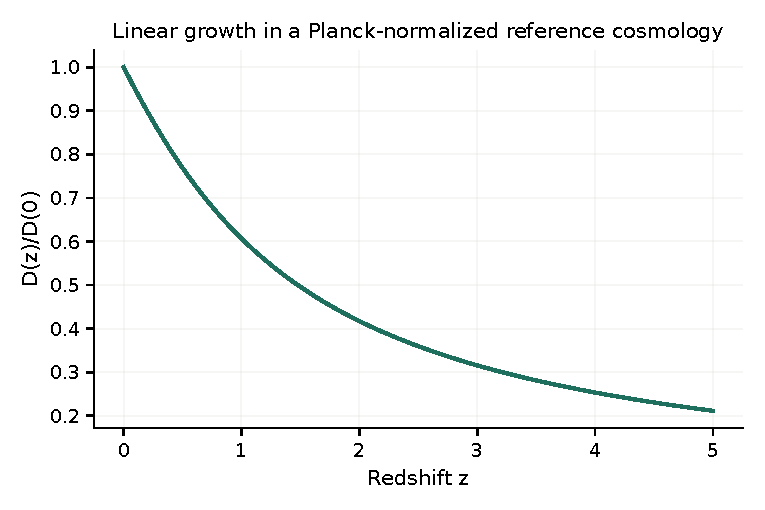
\includegraphics[width=.78\linewidth]{figures/growth_reference.pdf}\caption{Reference linear growth obtained from Eq.~\eqref{eq:growth}; the background and normalization are the stated Planck reference inputs.}\end{figure}

\subsubsection{A smooth matter-power reference spectrum}
The linear spectrum takes the form
\begin{equation}\label{eq:pk}
P_m(k,z)=A\,k^{n_s}T^2(k)D^2(z).
\end{equation}
For an inexpensive, explicitly approximate transfer calculation we use the baryon-corrected BBKS/Sugiyama smooth shape \cite{BBKS,Sugiyama}:
\begin{align}
T(q)&=\frac{\ln(1+2.34q)}{2.34q}
\bigl[1+3.89q+(16.1q)^2+(5.46q)^3+(6.71q)^4\bigr]^{-1/4},\\
q&=k/(h\Gamma_{\rm eff}),\quad
\Gamma_{\rm eff}=\Om_mh\exp\{-\Om_b[1+\sqrt{2h}/\Om_m]\},
\end{align}
Here $k$ is measured in $\Mp^{-1}$, as in the numerical implementation. The normalization is fixed by
\begin{equation}
\sigma_R^2=\frac{1}{2\pi^2}\int_0^\infty k^2P_m(k)W^2(kR)\dd k,\quad
W(x)=3\frac{\sin x-x\cos x}{x^3},
\quad \sigma_{8h^{-1}\Mp}=0.811.
\end{equation}
The numerical spectrum reproduces the supplied $\sigma_8$ under the stated physical-unit convention. BBKS describes a smooth linear transfer shape. Resolved acoustic features, nonlinear evolution and baryonic corrections belong to the corresponding Einstein--Boltzmann and matter-evolution model used in a survey likelihood.

\begin{figure}[t]\centering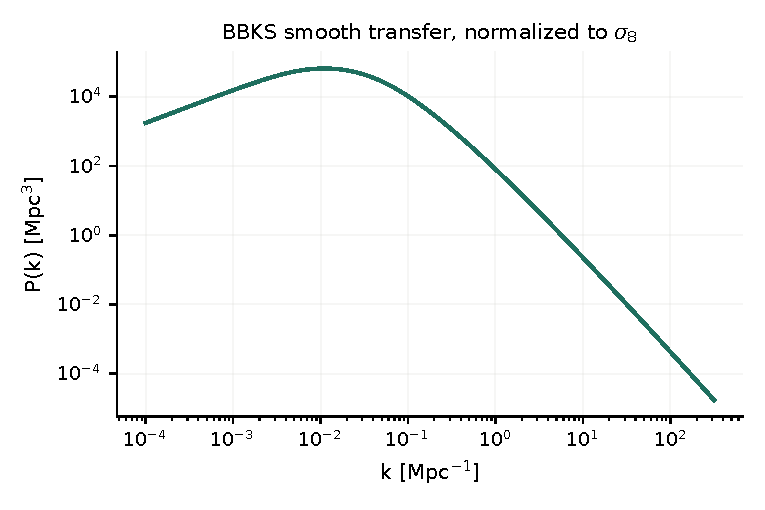
\includegraphics[width=.8\linewidth]{figures/matter_power_reference.pdf}\caption{Smooth BBKS-type reference spectrum normalized by the observed $\sigma_8$. The curve resolves the broad turnover in the smooth-transfer approximation.}\end{figure}

\subsection{Halo dynamics, mass functions, and galaxy populations}

\subsubsection{Halo abundance}\label{sec:halo-abundance}
For the Gaussian spherical-collapse reference with linear threshold $\delta_c=1.686$, the Press--Schechter estimate is
\begin{equation}
\frac{\dd n}{\dd\ln M}=\sqrt{\frac2\pi}\frac{\bar\rho_m}{M}
\frac{\delta_c}{\sigma(M)}\left|\frac{\dd\ln\sigma}{\dd\ln M}\right|
\exp\left[-\frac{\delta_c^2}{2\sigma^2(M)}\right].
\end{equation}
At $z=0$, the smooth reference spectrum gives $\dd n/\dd\ln M\simeq2.491\times10^{-3}$ Mpc$^{-3}$ at $M=10^{12}\msun$ and $2.704\times10^{-5}$ Mpc$^{-3}$ at $M=10^{14}\msun$. These are Press--Schechter estimates for the stated Gaussian-collapse and transfer assumptions \cite{PressSchechter,ShethTormen}. Survey counts also depend on the mass definition, selection function, cosmic variance, redshift-space mapping and halo occupation.

\begin{figure}[t]\centering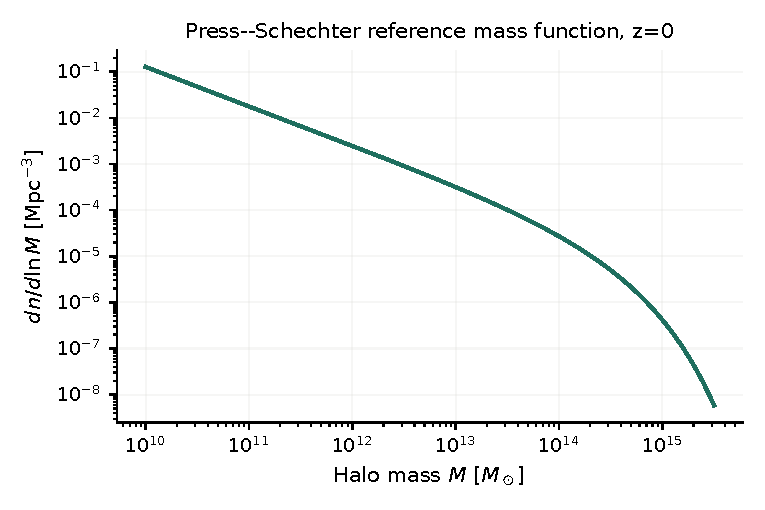
\includegraphics[width=.8\linewidth]{figures/halo_mass_function.pdf}\caption{Reference Press--Schechter halo abundance inferred from the smooth spectrum.}\end{figure}

\subsubsection{A radiation-consistent spherical-overdensity computation}\label{sec:spherical-collapse}
A uniform overdense region of fixed mass $M$ evolves in a smooth-$\Lambda$ background according to
\begin{equation}
\ddot R=-\frac{GM}{R^2}-\Omega_{r0}H_0^2a^{-4}R+\Omega_{\Lambda0}H_0^2R.
\end{equation}
Starting at $a_i=0.01$ with mass $M=10^{14}\msun$, $\delta_i=0.040$, radius fixed by mass conservation, and specified density-derivative initial velocity $\dot R_i=H_iR_i[1-\delta_i/(3(1+\delta_i))]$, the isolated top-hat reaches $R=0.01$ Mpc at $a=0.4614218$ in the reference background. The prescribed initial density derivative is $\delta_i^{\prime}=\delta_i$. The homogeneous radiation term is required by the same expansion background: setting $\delta_i=0$ recovers $R\propto a$. An independent density-contrast equation verifies the quoted threshold. The result describes one nonlinear, homogeneous overdensity with the stated initial data. Virial concentration, substructure and cosmological halo counts refer to distinct spatial observables.

\begin{figure}[t]\centering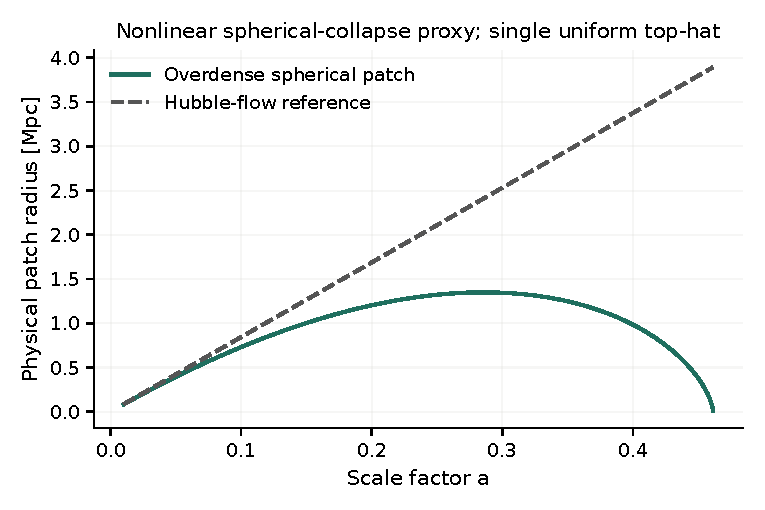
\includegraphics[width=.8\linewidth]{figures/spherical_collapse_reference.pdf}\caption{Numerical integration of an isolated spherical top-hat, compared with expansion at the background Hubble rate. The event is defined by the stated physical-radius threshold.}\end{figure}

\subsubsection{A transparent stellar-mass mapping}\label{sec:stellar-map}
The formation of observable galaxies requires star formation, feedback, metal enrichment, gas cooling, dust, and selection effects. For the limited purpose of illustrating the halo-to-stellar conversion, take
\begin{equation}
M_\star=\varepsilon_\star\frac{\Om_b}{\Om_m}M_h,
\quad \varepsilon_\star=0.05,\qquad
\phi_\star(M_\star)=\frac{\dd n}{\dd\log_{10}M_h}\left|\frac{\dd\log_{10}M_h}{\dd\log_{10}M_\star}\right|.
\end{equation}
For $M_h=10^{12}\msun$ the chosen constant-efficiency model gives $M_\star=7.816\times10^9\msun$. The chosen constant efficiency defines a deterministic halo-to-stellar mapping. Survey predictions extend it with scatter and a redshift-dependent star-formation model. Statistical galaxy clustering requires $P_g(k,z)=b_g^2(k,z)P_m(k,z)$ with a computed halo occupation or bias model and a likelihood against spectroscopic data. For example, the constant illustrative bias $b_g=1.5$ and the smooth linear spectrum yield
\begin{equation}
\xi_g(r)=\frac{b_g^2}{2\pi^2}\int_0^\infty k^2P_m(k,0)\frac{\sin kr}{kr}\dd k,
\quad \xi_g(10\,\Mp)=1.462405,\quad\xi_g(20\,\Mp)=0.466138.
\end{equation}
The oscillatory sine transform is evaluated adaptively over $0<k<\infty$, using a quadrature that resolves the oscillatory kernel. These values inherit the selected bias and observational normalization, and the smooth transfer sets their approximation domain separately from a resolved BAO calculation.

\begin{figure}[t]\centering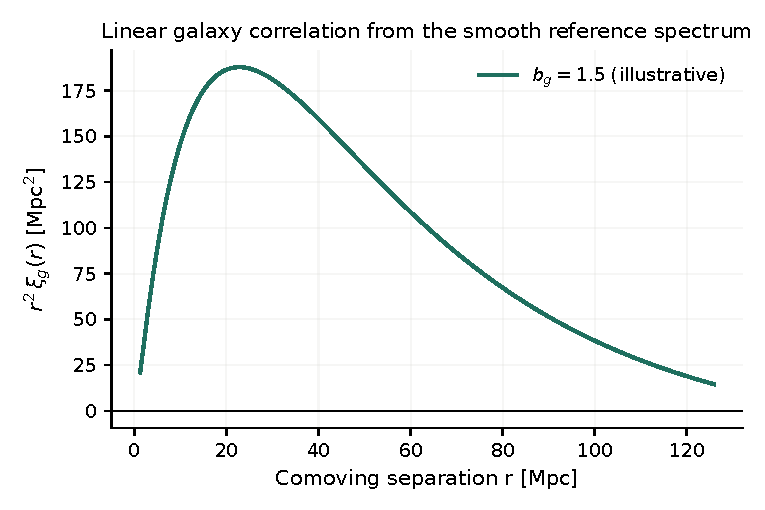
\includegraphics[width=.78\linewidth]{figures/galaxy_correlation_reference.pdf}\caption{Linear real-space galaxy correlation for a selected constant bias and BBKS smooth transfer. The observable is the real-space correlation before redshift-space and survey-window mapping.}\end{figure}

\begin{figure}[t]\centering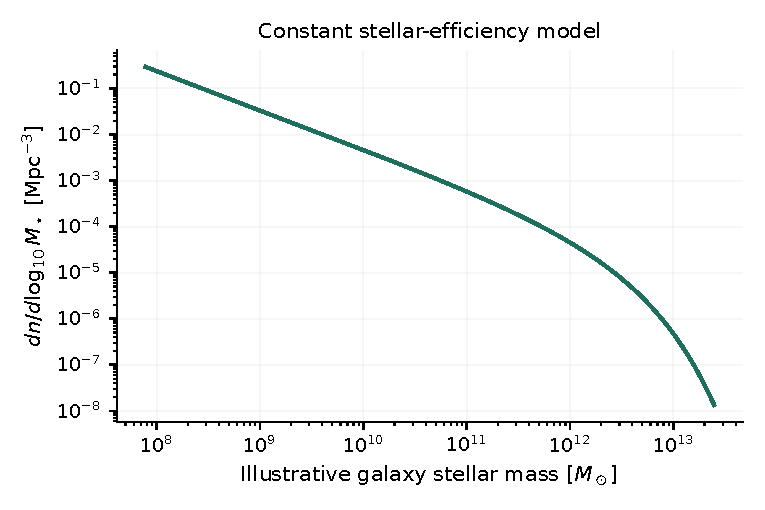
\includegraphics[width=.8\linewidth]{figures/stellar_mass_function.pdf}\caption{Stellar-mass function from a constant, explicitly chosen halo-to-stellar efficiency. The efficiency and background are independent inputs to this illustrative population model.}\end{figure}

\subsection{A three-dimensional gravitational clustering experiment}
\label{sec:pm3d}
The preceding halo calculation concerned a single spherical overdensity. To test gravitational clustering with spatially varying forces we additionally solved an explicit three-dimensional periodic particle--mesh (PM) system. The prescribed initial field defines a deterministic numerical experiment.

Let $\mathbf x$ be comoving coordinates in a periodic cube and $u=\ln a$. For pressureless particles in a flat matter-plus-$\Lambda$ background, the comoving evolution equations are
\begin{align}
\mathbf x'&=\mathbf v,\\
\mathbf v'&=-\left(2+\frac{H'}{H}\right)\mathbf v
-\frac32\Omega_m(a)\boldsymbol\nabla\nabla^{-2}\delta,
\qquad\delta=\frac{\rho-\bar\rho}{\bar\rho}.
\label{eq:pm}
\end{align}
We assigned and interpolated particle densities using cloud-in-cell weights, solved the periodic Poisson problem with a Fourier transform and advanced Eq.~\eqref{eq:pm} with a second-order midpoint integrator in $u$. The $k=0$ mode is set to zero, fixing the homogeneous potential gauge. The calculation uses $32^3$ equal-mass particles on a $32^3$ grid in a $100\,h^{-1}\,\mathrm{Mpc}$ box with 300 steps from $a=0.05$ to 1. The deliberately simple Zel'dovich initial displacement is a superposition of three coherent orthogonal plane waves with present-epoch linearly extrapolated amplitude 1.1. These three waves specify a coherent deterministic field.

The RMS grid-density contrast grows from $0.08547$ at $a=0.05$ to $3.1436$ at $a\approx0.5$ and $10.4690$ at $a=1$, with a final peak cell contrast of $1484.3$. The assignment conserves total particle mass to floating-point accuracy, and the deposited grid has mean $\langle\delta\rangle\simeq0$ at each stored epoch. These large cell contrasts follow from coherent nonlinear collapse and depend strongly on the selected particle and force resolution. Repeating the integration with 200 rather than 300 time steps changes the final grid RMS contrast by 0.25\% and the peak by 0.42\%; this comparison measures time discretization at fixed spatial resolution. The density statistics refer to this mesh and coherent initial field. Cosmological halo statistics additionally depend on the primordial ensemble, transfer function, box and force resolution, halo definition and baryonic dynamics.

\begin{figure}[t]
\centering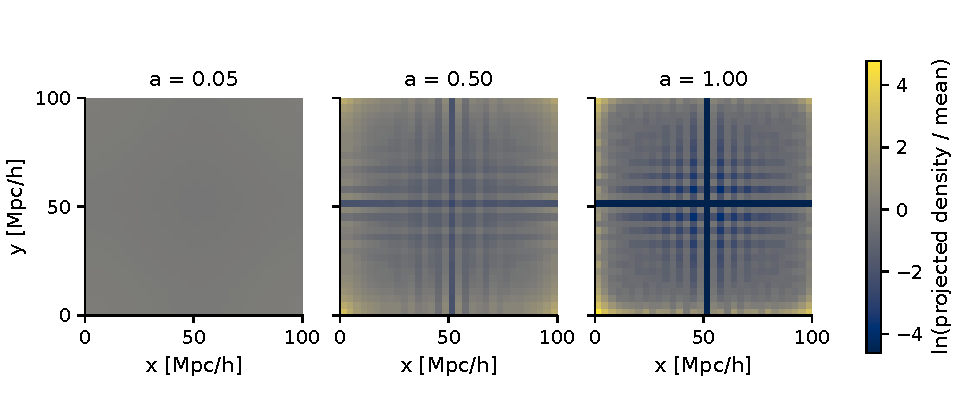
\includegraphics[width=\linewidth]{figures/particle_mesh_3d.pdf}
\caption{Evolution of the projected density in the numerical 3-D particle--mesh test at early, intermediate and late scale factors. The initial field contains coherent plane waves. All panels use the same logarithmic projected-density scale, with a display floor of 0.01 times the mean density.}
\end{figure}

\subsection{A solvable gas-regulator model for the stellar component}
\label{sec:gasreg}
A gas reservoir connects an imposed halo-accretion history to stellar growth. Suppose a halo accretes mass at a constant rate $\dot M_h$, a fraction $f_b$ reaches a gas reservoir, outflows remove $\eta_w\psi$, a fraction $\mathcal R$ of newly formed stellar mass is returned promptly, and the star formation law is $\psi=\epsilon_*M_g/t_d$. Then
\begin{equation}
\dot M_g=f_b\dot M_h-(1-\mathcal R+\eta_w)\frac{\epsilon_*}{t_d}M_g,
\qquad \dot M_*= (1-\mathcal R)\frac{\epsilon_*}{t_d}M_g.
\label{eq:gas-ode}
\end{equation}
For initially empty reservoirs, constant coefficients, $t_d>0$, $\epsilon_*>0$, $\eta_w\geq0$ and $0\leq\mathcal R<1$, let $\lambda=(1-\mathcal R+\eta_w)\epsilon_*/t_d>0$. The unique solution is
\begin{align}
M_g(t)&=\frac{f_b\dot M_h}{\lambda}\left(1-e^{-\lambda t}\right),\\
M_*(t)&=\frac{(1-\mathcal R)f_b\dot M_h}{1-\mathcal R+\eta_w}
\left[t-\frac{1-e^{-\lambda t}}{\lambda}\right],\\
\psi(t)&=\frac{f_b\dot M_h}{1-\mathcal R+\eta_w}\left(1-e^{-\lambda t}\right).
\label{eq:gas-sol}
\end{align}
The continuous limit $\epsilon_*\to0$ gives $M_g=f_b\dot M_h t$, $M_*=0$ and $\psi=0$. For the explicitly selected values $\dot M_h=50\,M_\odot\,\mathrm{yr}^{-1}$, $f_b=0.15633$, $\epsilon_*=0.05$, $t_d=0.1\,\mathrm{Gyr}$, $\mathcal R=0.4$, $\eta_w=1$ and $t=3\,\mathrm{Gyr}$, the solution gives $M_g=8.8841\times10^9M_\odot$, $M_*=5.4619\times10^9M_\odot$ and $\psi=4.4421\,M_\odot\,\mathrm{yr}^{-1}$. These are conditional predictions of the adopted gas-regulator model. The baryon fraction is computed from the previously adopted Planck reference parameters; the efficiencies and accretion history are chosen inputs. The calculation describes one well-mixed reservoir with instantaneous recycling and the stated constant coefficients. Resolved cooling, enrichment and radiative feedback define additional physical degrees of freedom in a spatial galaxy model.


\subsubsection{Time-dependent inflow and the baryon balance}
The gas-reservoir equation also has an exact solution for time-dependent coefficients. Let $I(t)=f_b(t)\dot M_h(t)$, $k_*(t)=\epsilon_*(t)/t_d(t)$ and $\lambda(t)=[1-\mathcal R(t)+\eta_w(t)]k_*(t)$, with $I,k_*,\eta_w\geq0$ and $0\leq\mathcal R<1$. For integrable coefficients, define $L(t)=\int_0^t\lambda(u)\dd u$. The integrating factor gives
\begin{equation}\label{eq:gas-green}
M_g(t)=M_g(0)e^{-L(t)}+\int_0^t I(s)e^{-[L(t)-L(s)]}\dd s.
\end{equation}
This is the unique solution and is nonnegative for nonnegative initial gas mass. The stellar and cumulative wind masses follow by integration of $(1-\mathcal R)k_*M_g$ and $\eta_wk_*M_g$, respectively. Adding the three equations proves the exact balance
\begin{equation}\label{eq:gas-balance}
M_g(t)+M_*(t)+M_w(t)
=M_g(0)+M_*(0)+M_w(0)+\int_0^t I(s)\dd s.
\end{equation}
For constant return and loading factors and initially empty reservoirs, $M_w=\eta_wM_* /(1-\mathcal R)$. The selected three-gigayear example therefore has $M_w=9.10314\times10^9M_\odot$ and cumulative gas inflow $2.34491\times10^{10}M_\odot$, consistent with the gas and stellar masses above. Equation~\eqref{eq:gas-green} shows explicitly how the consumption and outflow rates set the memory of the accretion history.

\section{Lensing and joint scalar metric observables}\label{sec:lensing}

\subsection{Deflection, convergence, shear, and mass maps}
For an isotropic weak-field metric in Newtonian gauge,
\begin{equation}
\dd s^2=-(1+2\Psi/c^2)c^2\dd t^2+a^2(1-2\Phi/c^2)\dd\mathbf x^2,
\end{equation}
the lensing potential probes $(\Phi+\Psi)/2$. The matter-to-metric response specifies both potentials and their gravitational slip $\eta=\Phi/\Psi$. When the standard weak-field limit holds, the thin-lens relations are
\begin{align}
\bm\alpha(\bm\theta)&=\frac{1}{c^2}\frac{D_{ls}}{D_s}\int\nabla_\perp(\Phi+\Psi)\,\dd\ell,\\
\kappa(\bm\theta)&=\frac12\nabla_\theta^2\psi(\bm\theta)=\frac{\Sigma_{\rm mass}}{\Sigma_{\rm crit}},\qquad
\Sigma_{\rm crit}=\frac{c^2}{4\pi G}\frac{D_s}{D_lD_{ls}},\\
\gamma_1&=\tfrac12(\psi_{,11}-\psi_{,22}),\qquad \gamma_2=\psi_{,12}.
\end{align}
Here $\Sigma_{\rm mass}$ denotes projected mass per area; the dimensionless response $\Sigma$ is defined in Section~\ref{sec:metric-scalar-joint}. For $\Phi=\Psi$, integration along a straight ray gives the physical point-mass bending angle $4GM/(bc^2)$. The reduced angular deflection $\bm\alpha$ includes the additional distance ratio $D_{ls}/D_s$. The angular and surface-density conventions are fixed in the source code.

\subsection{Galaxy strong lens and time delay}\label{sec:sis}
For a singular isothermal sphere with line-of-sight velocity dispersion $\sigma_v$,
\begin{equation}
\theta_E=4\pi\left(\frac{\sigma_v}{c}\right)^2\frac{D_{ls}}{D_s},\quad
\kappa(\theta)=\gamma_t(\theta)=\frac{\theta_E}{2\theta}.
\end{equation}
The arrival-time surface gives $\Delta t=(1+z_l)(D_lD_s/cD_{ls})\,\Delta[\frac12|\bm\theta-\bm\beta|^2-\psi(\bm\theta)]$. For $z_l=0.3$, $z_s=1$, $\sigma_v=220$ km s$^{-1}$ and $\beta=\theta_E/2$, the reference geometry yields
\begin{equation}
\boxed{\theta_E=0.8884\ \mathrm{arcsec},\qquad |\Delta t|=42.93\ \mathrm{days}.}
\end{equation}
The source offset and velocity dispersion are chosen examples. The values are conditional on this lens geometry, dispersion and source position.

\subsection{Cluster lens, convergence map, and statistical shear}\label{sec:cluster-lensing}
Take a Navarro--Frenk--White density profile \cite{NFW}, $\rho(r)=\rho_s/[ (r/r_s)(1+r/r_s)^2 ]$, with $M_{200}=10^{14}\msun$, concentration $c_{200}=5$, and lens/source redshifts as above. The reference calculation gives $r_{200}=0.8826$ Mpc, and at projected radius $R=0.1$ Mpc,
\begin{equation}
\boxed{\kappa(0.1\,\Mp)=0.1197,\qquad\gamma_t(0.1\,\Mp)=0.0708.}
\end{equation}
An idealized $10^{15}\msun$ NFW cluster with $c_{200}=4$ has a tangential critical radius $R_t=0.02469$ Mpc, corresponding to $\theta_t=5.35$ arcsec for this geometry, under the adopted spherical profile and background. This last quantity is profile-dependent.

\begin{figure}[t]\centering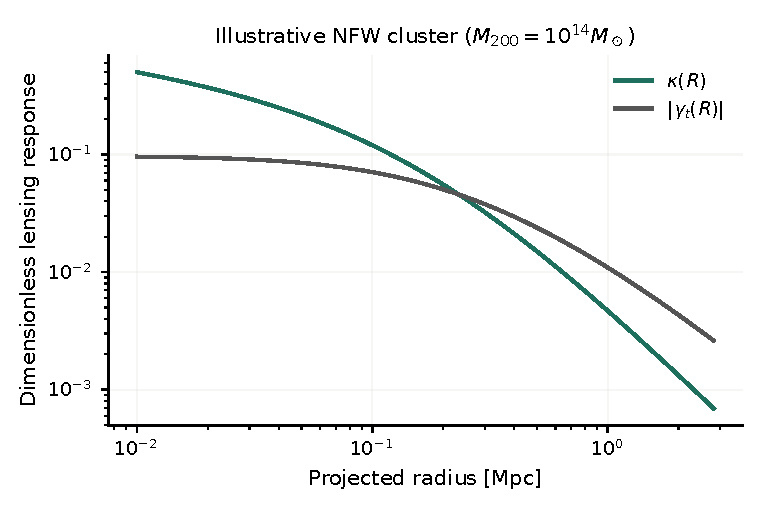
\includegraphics[width=.75\linewidth]{figures/cluster_lensing_reference.pdf}\caption{Spherically averaged NFW lens convergence and tangential shear for the stated analytic reference cluster.}\end{figure}

\begin{figure}[t]\centering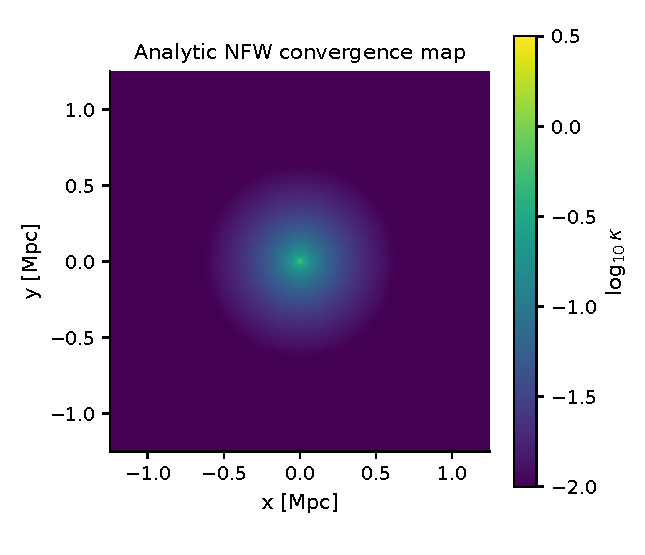
\includegraphics[width=.67\linewidth]{figures/cluster_kappa_map.pdf}\caption{Projected NFW convergence map computed analytically. The map is the projection of the specified spherical analytic density profile.}\end{figure}

For normalized comoving source distributions $n_i(\chi_s)$, define the Weyl-potential lensing efficiency
\begin{equation}
q_i(\chi)=\int_\chi^{\chi_H}\dd\chi_s\,n_i(\chi_s)\frac{\chi_s-\chi}{\chi_s\chi},
\qquad \int_0^{\chi_H}n_i(\chi_s)\,\dd\chi_s=1.
\end{equation}
Writing $P_{\Phi+\Psi}$ for the three-dimensional power spectrum of the \emph{dimensional} sum of the two Newtonian-gauge potentials, the Born--Limber angular convergence spectrum is
\begin{equation}\label{eq:weyl-limber-corrected}
C_\ell^{\kappa_i\kappa_j}\simeq \frac{[\ell(\ell+1)]^2}{4c^4}
\int_0^{\chi_H}\frac{\dd\chi}{\chi^2}\,q_i(\chi)q_j(\chi)
P_{\Phi+\Psi}\!\left(\frac{\ell+1/2}{\chi},z(\chi)\right).
\end{equation}
The angular-derivative factor and powers of $c$ are essential when the spectrum is defined for the dimensional Weyl potentials rather than the matter density. For $\Phi=\Psi$ and the standard Poisson equation, its large-$\ell$ limit agrees with the matter-spectrum convergence integral in Eq.~\eqref{eq:clkk}. A survey comparison additionally includes calibrated redshift distributions, intrinsic alignments, baryonic and nonlinear effects, masks, selection functions, and covariance.

\subsection{A computed angular convergence spectrum}
\label{sec:shear}
The standard weak-lensing limit gives a tractable \emph{angular} statistic in addition to the analytic galaxy and cluster lenses calculated above. For a thin source plane at comoving distance $\chi_s$, the first-order convergence kernel in flat GR is
\begin{equation}
W_\kappa(\chi)=\frac{3\Om_mH_0^2}{2c^2}\frac{\chi}{a(\chi)}\frac{\chi_s-\chi}{\chi_s},\qquad 0<\chi<\chi_s.
\end{equation}
Under the Born approximation and Limber correspondence $k=(\ell+1/2)/\chi$, the E-mode convergence power is
\begin{equation}\label{eq:clkk}
\boxed{C_\ell^{\kappa\kappa}=\int_0^{\chi_s}\frac{\dd\chi}{\chi^2}\,W_\kappa^2(\chi)P_\delta\!\left(\frac{\ell+1/2}{\chi},z(\chi)\right).}
\end{equation}
For a reference source redshift $z_s=1$, smooth BBKS matter transfer, observed $\sigma_8$ normalization and the linear growth solution in Section~\ref{sec:structure}, direct quadrature gives:
\begin{equation}\label{eq:numshear}
\boxed{C_{50}^{\kappa\kappa}=1.701\times10^{-8},\quad
C_{200}^{\kappa\kappa}=2.544\times10^{-9},\quad
C_{1000}^{\kappa\kappa}=9.18350\times10^{-11}.}
\end{equation}
The source distance and complete multipole grid are saved in \texttt{closure\_results.json}. These outputs evaluate the single-plane linear GR integral with its stated smooth transfer and normalization. Precision shear inference further includes nonlinear clustering, intrinsic alignments, source-redshift distributions, baryonic effects, photometric calibration and the physical Weyl response.

\begin{figure}[t]\centering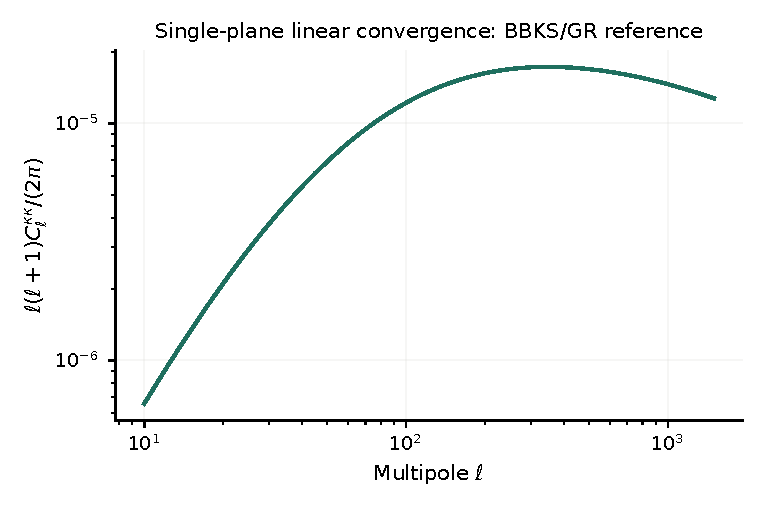
\includegraphics[width=.8\linewidth]{figures/linear_cosmic_shear_limber.pdf}
\caption{Angular convergence power for a source plane at $z_s=1$, evaluated with the linear GR growth and smooth transfer of the reference model. The displayed quantity is $\ell(\ell+1)C_\ell^{\kappa\kappa}/(2\pi)$.}\label{fig:angular-convergence}
\end{figure}

\subsubsection{Metric-response consistency test}
The general weak-field deflection probes the sum of the potentials with the $1/c^2$ convention given above. Equation~\eqref{eq:clkk} adopts the GR response $\Phi=\Psi$. A general scalar response enters the same observable through the density-to-Weyl transfer in Eq.~\eqref{eq:weyl-limber-corrected}.

\subsection{Growth, slip and the velocity--lensing ratio}
\label{sec:metric-scalar-joint}
Cosmological scalar perturbations probe an additional sector of the metric response. At subhorizon scales, in the quasistatic regime and in a specified gauge, a minimally useful parameterization of the scalar response is
\begin{align}
-k^2\Psi&=4\pi G a^2\bar\rho_m\,\mu(k,a)\,\delta_m,\\
\Phi&=\eta(k,a)\Psi,\qquad
\Sigma(k,a)=\frac{\mu(k,a)[1+\eta(k,a)]}{2}.
\end{align}
The single field $\Psi$ controls nonrelativistic acceleration, whereas $\Phi+\Psi$ controls weak and strong lensing. In the general-relativistic limit $\mu=\eta=\Sigma=1$. In the QICT description, $\mu$ and $\eta$ are defined by the scalar density and metric kernels of the same renormalized state used for the tensor response.

For pressureless matter, negligible anisotropic stress in the matter sector and a quasistatic conserved fluid, the continuity and Euler equations give
\begin{equation}
D_k''+\left(2+\frac{H'}{H}\right)D_k'-\frac32\Omega_m(a)\mu(k,a)D_k=0,
\qquad {}'=\frac{\dd}{\dd\ln a}.
\label{eq:joint-growth}
\end{equation}
For physical peculiar velocity $\mathbf v_m$ and comoving gradient $\nabla$, define $\theta_m=\nabla\cdot\mathbf v_m/(aH)$. With $f=D_k'/D_k$, the linear continuity relation gives $\theta_m=-f\delta_m$. The ideal velocity--lensing statistic obeys \cite{Zhang07}
\begin{equation}
\boxed{E_G(k,z)=\frac{\Omega_{m0}\,\Sigma(k,z)}{f(k,z)}.}\label{eq:eg-null}
\end{equation}
The relation follows from $-k^2(\Phi+\Psi)=3H_0^2\Omega_{m0}\Sigma\delta_m/a$, together with the continuity relation, after common normalization factors have been removed. It is independent of the matter-power amplitude in the idealized deterministic, scale-matched limit. Galaxy bias, redshift-space distortions, nonlinear contributions and observational window functions enter the covariance and window of a measured estimator.

The baseline $\Omega_{m0}=0.315$ yields $f(0.5)=0.76087$ and $E_G(0.5)=0.41400$ from a direct integration of Eq.~\eqref{eq:joint-growth}. For an explicit alternative scalar-response \emph{example}, $\mu=1.05$ and $\eta=0.90$ give $\Sigma=0.9975$, $f(0.5)=0.78363$ and $E_G(0.5)=0.40097$. If both growth histories have the same density amplitude at $a=0.01$ (and their growing matter-era solutions are separately imposed), the equal-time three-dimensional Weyl-potential power at $z=0.5$ changes by a factor $1.2683337$. The angular convergence spectrum instead integrates the changed growth along the line of sight. For a source plane at $z_s=1$, the ratios $C_\ell^{\kappa\kappa}(\mu=1.05,\eta=0.90)/C_\ell^{\kappa\kappa}(\mathrm{GR})$ are $1.2737472$, $1.2709505$ and $1.2695077$ at $\ell=50,200,1000$, respectively. Both use the same initial density amplitude at $a=0.01$ and the same background geometry. This exercise shows how a near-standard lensing strength can coexist with a different growth history. The values of $\mu$ and $\eta$ are selected inputs to this response test. The full calculation and normalization convention appear in the attached script.


\subsection{Direct inversion of the scalar response}
\label{sec:growth-inversion}
The growth equation and the velocity--lensing ratio also determine an inverse relation. At fixed wavenumber, assume conserved pressureless matter, a specified background $H(a)$ and $\Omega_{m0}$, the quasistatic scalar response of Eq.~\eqref{eq:joint-growth}, and $f\neq0$, $\mu\neq0$. Then
\begin{equation}\label{eq:growth-inversion}
\boxed{\begin{aligned}
\mu(k,a)&=\frac{2}{3\Omega_m(a)}
\left[f'+f^2+\left(2+\frac{H'}H\right)f\right],\\
\eta(k,a)&=\frac{2f(k,a)E_G(k,a)}{\Omega_{m0}\mu(k,a)}-1.
\end{aligned}}
\end{equation}
For the first identity, divide the growth equation by $D$ and use $D''/D=f'+f^2$. The second follows by substituting $\Sigma=\mu(1+\eta)/2$ into Eq.~\eqref{eq:eg-null}. An overall normalization of $D$ cancels from both expressions. In a numerical check, differentiating independently integrated growth histories recovers $(\mu,\eta)=(1,1)$ and $(1.05,0.90)$ with absolute errors below $2\times10^{-10}$. These are tests of the inversion under its stated assumptions. An observational application supplies the covariance of the reconstructed derivative, the background and the scale-matched velocity--lensing statistic.

\section{CMB transfer observables and initial-state dependence}\label{sec:cmb}

\subsection{Acoustic scale and thermal history}\label{sec:acoustic-scale}
For the Planck-normalized spatially flat reference model, photon-baryon sound speed and sound horizon obey
\begin{align}
c_s(a)&=\frac{c}{\sqrt{3[1+R_b(a)]}},\qquad R_b(a)=\frac{3\Om_b}{4\Om_\gamma}a,\\
r_s(z_*)&=\int_0^{a_*}\frac{c_s(a)}{a^2H(a)}\dd a,\\
D_M(z_*)&=c\int_0^{z_*}\frac{\dd z}{H(z)},\quad \theta_*=\frac{r_s(z_*)}{D_M(z_*)},\quad \ell_A=\frac\pi{\theta_*}.
\end{align}
Taking $z_*=1089.92$ as an \emph{external recombination input}, our integrations return
\begin{equation}
\boxed{\begin{aligned}
r_s(z_*)&=144.294\ \Mp,&D_M(z_*)&=13864.38\ \Mp,\\
100\theta_*&=1.04075,&\ell_A&=301.86.
\end{aligned}}
\end{equation}
The inferred Planck acoustic-angle reference is $100\theta_*=1.0411\pm0.0003$ \cite{Planck}. The present value is conditional on the supplied $z_*$, densities and $H_0$, and tests this approximate background geometry. The quantity $\ell_A$ is the acoustic spacing; radiation driving and phase shifts place the first TT peak near $\ell\sim220$.

\subsection{Temperature, polarization, and lensing spectra}\label{sec:cmb-state}
Temperature and polarization observables combine their transfer functions with a specified primordial state. A convenient primordial parameterization is
\begin{equation}
\mathcal P_{\mathcal R}(k)=A_s\left(\frac{k}{k_0}\right)^{n_s-1+\frac12\alpha_s\ln(k/k_0)+\cdots}.
\end{equation}
The baryon loading determines odd/even peak heights, gravitational potential evolution and neutrino free streaming control acoustic phases, photon diffusion causes Silk damping, and Thomson scattering generates polarization. A kinetic recombination solution evolves the ionization fractions and matter temperature together. Reionization and optical depth $\tau_{\rm reio}$ then modify large-scale E modes and damp primary small-scale anisotropies. The observational Planck baseline gives $\Om_bh^2\simeq0.02237$, $\Om_ch^2\simeq0.1200$, $n_s\simeq0.965$ and $\tau_{\rm reio}\simeq0.054$ \cite{Planck}.
Hydrogen Saha equilibrium gives an explicit thermodynamic reference:
\begin{equation}
\frac{x_e^2}{1-x_e}=\frac1{n_H}\left(\frac{m_ek_BT}{2\pi\hbar^2}\right)^{3/2}\exp\!\left[-\frac{13.5984\,\mathrm{eV}}{k_BT}\right].
\end{equation}
For $Y_p=0.245$ and $T_0=2.7255$ K, the equilibrium solution has $x_e=1/2$ at $z\simeq1369$ and $x_e(z_*)\simeq0.00376$. These values describe the equilibrium ionization fraction. Delayed recombination, residual electrons and helium populations are governed by the multilevel-atom rate equations. Their electron density determines the Thomson visibility and the kinetic last-scattering distribution.

\begin{figure}[t]\centering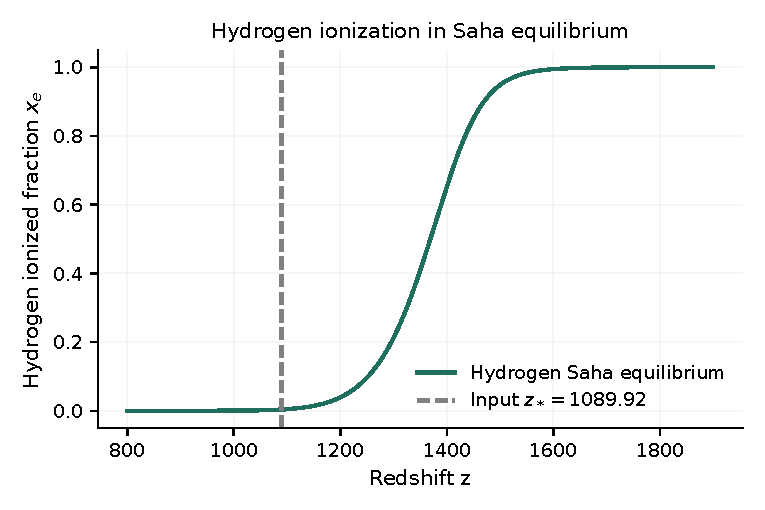
\includegraphics[width=.79\linewidth]{figures/saha_ionization_reference.pdf}\caption{Hydrogen equilibrium ionization history and the independently imposed reference last-scattering redshift. The plotted curve describes Saha equilibrium; visibility is defined by the kinetic electron density.}\end{figure}

The calculated CMB numbers describe acoustic geometry and the equilibrium reference. The temperature, polarization and lensing spectra are analytic functionals of the separately specified primordial measure and kinetic transfer functions.

\subsection{Line-of-sight sources, polarization and diffusion}
\label{sec:cmb-hierarchy}
CMB temperature and polarization power depend on dynamical sources along the photon trajectory. For each Fourier mode, the Einstein--Boltzmann hierarchy evolves the metric and matter fluids, photon temperature and polarization multipoles, baryon velocity, neutrinos, and the recombination visibility function. In the following transfer formulas, conformal time and distance are expressed in units with $c=1$. Under scalar adiabatic initial conditions, the conventional line-of-sight construction may be written \cite{Ma95,Seljak96}
\begin{align}
\Delta_\ell^{T}(k)&=\int_0^{\eta_0}\dd\eta\,S_T(k,\eta)j_\ell[k(\eta_0-\eta)],\\
\Delta_\ell^{E}(k)&=\sqrt{\frac{(\ell+2)!}{(\ell-2)!}}
\int_0^{\eta_0}\dd\eta\,\frac{3g(\eta)\Pi(k,\eta)}{4[k(\eta_0-\eta)]^2}
 j_\ell[k(\eta_0-\eta)],\\
C_\ell^{XY}&=4\pi\int\dd\ln k\,\mathcal P_{\mathcal R}(k)\,\Delta_\ell^{X}(k)\Delta_\ell^{Y}(k),
\qquad X,Y\in\{T,E\},
\label{eq:cl}
\end{align}
The E-mode expression applies for $\ell\geq2$. The transfer $\Delta_\ell^T$ refers to $\Delta T/T_0$ and polarization is in the same temperature normalization, so these $C_\ell$ are dimensionless; multiplication by $(10^6T_0)^2$ gives $\mu\mathrm K^2$. Here $q(\eta)=a n_e\sigma_T>0$, $\tau(\eta)=\int_\eta^{\eta_0}q(\eta^{\prime})\dd\eta^{\prime}$ and $g(\eta)=q(\eta)e^{-\tau(\eta)}$ is the positive Thomson visibility and $\Pi$ is the photon quadrupole polarization source. The expressions include Sachs--Wolfe, integrated Sachs--Wolfe and Doppler terms through $S_T$ once those sources have been calculated. The primordial spectrum $\mathcal P_{\mathcal R}$ specifies the initial-state measure; its provenance is either a stated early-time QICT state or an external cosmological input.

In the tightly coupled epoch the baryon-to-photon inertia ratio $R=3\rho_b/(4\rho_\gamma)$ sets the adiabatic sound speed $c_s^2=1/[3(1+R)]$ in units $c=1$, and the diffusion damping scale is
\begin{equation}
 k_D^{-2}(\eta)=\int_0^\eta\frac{\dd\eta'}{6q(\eta^{\prime})(1+R)}
\left[\frac{R^2}{1+R}+\frac{16}{15}\right].
\label{eq:silk}
\end{equation}
The acoustic separation is approximately $\ell_A=\pi\chi_*/r_s(\eta_*)$; the individual TT peak positions differ from integer multiples of $\ell_A$ because of radiation driving, baryon loading, free-streaming species and projection. Relative peak heights encode the baryon density, matter--radiation equality and primordial tilt. Small-scale damping depends on the ionization history and the polarization collision source. Cosmic lensing remaps the primary sky through the scalar Weyl-potential power along the line of sight. The acoustic geometry and the full TT, TE and EE transfer functions thus represent distinct levels of the calculation.

For completeness, the same scalar metric gives the CMB lensing transfer explicitly. In a spatially flat background and the Born approximation, define $T_{\rm W}$ by $(\Phi+\Psi)(\mathbf k,\eta)=T_{\rm W}(k,\eta)\mathcal R_{\mathbf k}$ in the present $c=1$ convention. With the unobservable angular monopole subtracted inside the line-of-sight integral, the lensing potential and its transfer for $L\geq2$ satisfy \cite{Lewis06}
\begin{align}
\phi(\widehat{\mathbf n})&=-\int_0^{\chi_*}\dd\chi\,
\frac{\chi_*-\chi}{\chi_*\chi}(\Phi+\Psi)_{\rm aniso}(\chi\widehat{\mathbf n},\eta_0-\chi),\\
\Delta_L^\phi(k)&=-\int_0^{\chi_*}\dd\chi\,
\frac{\chi_*-\chi}{\chi_*\chi}T_{\rm W}(k,\eta_0-\chi)j_L(k\chi),\\
C_L^{\phi\phi}&=4\pi\int\dd\ln k\,
\mathcal P_{\mathcal R}(k)|\Delta_L^\phi(k)|^2.\label{eq:cmb-lensing-transfer}
\end{align}
The subscript $\mathrm{aniso}$ denotes subtraction of the angular mean at each distance. The observable deflection is $\nabla_{\widehat{\mathbf n}}\phi$. These relations follow by expanding the line-of-sight Weyl potential in spherical harmonics and applying the primordial covariance. They use the same metric transfer as the temperature and polarization calculation. Their evaluation requires the specified primordial state and transfer evolution.

The transfer integrals define the spectra for a given primordial measure, recombination history and metric response. Their positivity and the information retained by a finite set of angular quantities follow directly.


\subsection{Positivity and the information in finite angular spectra}
\label{sec:cmb-positive}
The transfer representation imposes an exact consistency condition on temperature, polarization and any additional linearly transferred field sharing the same primordial scalar source.
\begin{proposition}[Positive angular covariance]\label{prop:cmb-positive}
For $\mathcal P_{\mathcal R}(k)\geq0$ and square-integrable transfer functions, the matrix
\[
\mathsf C_\ell^{XY}=4\pi\int\dd\ln k\,
\mathcal P_{\mathcal R}(k)\Delta_\ell^X(k)\Delta_\ell^{Y*}(k)
\]
is positive semidefinite. In particular,
\begin{equation}\label{eq:cmb-cauchy}
C_\ell^{TT}\geq0,\qquad C_\ell^{EE}\geq0,\qquad
|C_\ell^{TE}|^2\leq C_\ell^{TT}C_\ell^{EE}.
\end{equation}
For positive diagonal entries, equality holds precisely when the two transfer functions are proportional almost everywhere with respect to the primordial measure.
\end{proposition}
\begin{proof}
For every vector $b$, the quadratic form $b^\dagger\mathsf C_\ell b$ is the integral of $4\pi\mathcal P_{\mathcal R}|\sum_Xb_X^*\Delta_\ell^X|^2$. Positivity and the two-dimensional principal minor give Eq.~\eqref{eq:cmb-cauchy}. Equality is the equality condition in the Cauchy--Schwarz inequality for the two transfer functions. The cross spectrum may have either sign.
\end{proof}

The primordial information retained by a finite set of spectra has an equally precise characterization. For fixed transfer functions, write $m$ measured angular quantities as $c_i=\int K_i(k)\mathcal P(k)\,\dd\ln k$. Suppose an admissible reference spectrum is bounded below by a positive constant on a compact interval. Choose $m+1$ smooth, linearly independent functions $b_j$ supported inside that interval. The $m\times(m+1)$ matrix $A_{ij}=\int K_i b_j\,\dd\ln k$ has a nonzero null vector $v$. Consequently
\begin{equation}\label{eq:primordial-null-family}
\mathcal P_\varepsilon(k)=\mathcal P_0(k)+\varepsilon\sum_{j=1}^{m+1}v_jb_j(k)
\end{equation}
gives the same $c_i$ for all $i$, while sufficiently small $|\varepsilon|$ preserves positivity. Thus finite angular information determines an equivalence class of primordial functions. A finite-dimensional primordial model, such as the power-law parameterization above, selects a specified subfamily for inference. The acoustic geometry, transfer dynamics and primordial measure remain individually defined constituents of each CMB prediction.

\section{Physical inference and uncertainty propagation}\label{sec:inference}
A specified microscopic model and its astrophysical environment define a joint data likelihood. Write $\vartheta$ for the microscopic coordinates and $\nu$ for nuisance parameters. For conditionally independent data subsets, with shared calibrations included in $\nu$,
\begin{equation}
\mathcal L_{\rm joint}(\vartheta,\nu)=\mathcal L_{\cmb}\mathcal L_{\rm BAO}
\mathcal L_{\rm galaxy}\mathcal L_{\rm shear}\mathcal L_{\rm direct}\mathcal L_{\gamma}\mathcal L_{\bar p}.
\end{equation}
Correlated subsets are described by their joint likelihood. A predictive test fixes $\vartheta$ from the operator construction or from measurements disjoint from the tested observables. Calibration against an abundance or a scattering limit instead defines an inverse problem, such as Eq.~\eqref{eq:widthinv} or Eq.~\eqref{eq:portalbound}.

The theoretical error distribution propagates source-moment uncertainties, regulator and volume matching, analytic continuation, interaction amplitudes, the primordial and reheating state, numerical integration, and astrophysical modelling. Their correlations enter a common covariance or a joint distribution. Numerical convergence quantifies the numerical component under the declared model assumptions. Observational covariance enters separately through the detector or survey likelihood.

\subsection{Particle and survey response functions}\label{sec:comparisonhierarchy}
The thermal collision kernel determines a relic abundance. The matched nucleon amplitude, local density and velocity distribution determine the direct-detection rate per detector mass,
\begin{equation}\label{eq:direct-count}
\frac{\dd R}{\dd E_R}=\frac{\rho_\chi}{m_\chi m_T}
\int_{v>v_{\min}}\dd^3v\,f_\oplus(\mathbf v)\,v
\frac{\dd\sigma_T}{\dd E_R}.
\end{equation}
Here $\rho_\chi$ is the local particle mass density, $m_T$ is the target-nucleus mass and $f_\oplus$ is normalized by $\int\dd^3v\,f_\oplus(\mathbf v)=1$. A detector with several target species uses their mass-fraction-weighted rates.
The LZ or XENONnT detector model maps this recoil spectrum through efficiencies, energy resolution and the signal-plus-background likelihood. The selected 40-GeV, $\lambda_{HS}=0.01$ point lies outside the published LZ allowed region under the stated full-local-abundance assumptions. A different source-defined candidate carries its own mass, vertex and local phase-space distribution. The XENONnT 3.1 tonne-year analysis quotes its minimum 90\% spin-independent limit near $1.7\times10^{-47}\,\mathrm{cm}^2$ at 30 GeV \cite{XENON25}; each candidate is compared at its own mass and interaction form.

Gamma-ray inference combines the annihilation rate, photon yield and target $J$-factor. Charged-particle inference additionally includes transport and secondary production. A galaxy-survey likelihood combines anisotropic clustering with bias, redshift-space distortions, selection functions and instrumental windows. DESI DR2 BAO distances constrain expansion histories in combination with other probes \cite{DESI25}. The QICT vacuum coefficient has the distinct operator definition in Eq.~\eqref{eq:matching}; its observational comparison is made through the resulting metric response and expansion history.

The explicit constructions in Propositions~\ref{prop:odd-nonidentification}, \ref{prop:energy-branch} and \ref{prop:interaction-data}, together with Eqs.~\eqref{eq:source-curvature}, \eqref{eq:momentum-sample-family} and \eqref{eq:primordial-null-family}, characterize the independent physical information in this inference problem. They establish precisely which extensions preserve the recorded observables. Each numerical value in the accompanying standalone prediction register is therefore associated with the data and assumptions that determine it.

\section{Conclusions}
Source moments identify a well-defined part of unitary dynamics. The exact boundary is the reducing cyclic source space: an exact flat Gram rank reconstructs it, a near-invariant first moment gives a quantitative approximation, and positive moment forms bound its spectral weight. The optimized atomic-weight hierarchy is sharp for the truncated problem. Under a certified angular gap, a degree-$N-1$ Chebyshev filter gives an exponential enclosure and controls the interchange of regulator and moment limits.

The C9 calculation makes the additional information in the operators explicit. Exact rational evaluation gives a zero-phase upper weight of $0.001956273015$ from thirteen R4 moments. Direct reconstruction recovers those moments from the joint stationary prescription. A separate outward-rounded spectral certificate proves exactly zero weight at that phase for the polar-unitary finite model at every supplied cutoff. It covers the complete relevant spectra and holds for every stationary state, with a quantified operator perturbation margin. The finite operator conclusion, the truncated-data extremum and the continuum convergence theorem thus have individually specified hypotheses and reproducible tests.

The response analysis separates quantities that enter different physical questions. Energy branches assign physical energies to transfer phases; multiparticle dynamics determine connected interactions; source-contact derivatives contribute to metric curvature. Their independence is established by explicit operator families. Positive finite Lehmann weights provide a convergent low-frequency expansion, alternating remainder bounds and global real-axis enclosures. The gravitational matching identities then relate physically normalized continuum coefficients to $G$, $\Lambda$ and the clock-independent ratio $\epsilon_0/\gamma_R^2$.

The thermal and cosmological results are equally explicit about their domains. A positive-source comparison bounds the late abundance, entropy conservation gives the decay yield with variable degrees of freedom, and differentiation fixes its reheating sensitivity. Growth and lensing recover the scalar response under conserved quasistatic matter dynamics. The gas solution obeys an exact baryon balance, while the CMB transfer measure gives positive angular covariances and a constructive characterization of finite primordial information. All numerical examples are reproduced from their stated inputs. Together, the proofs and calculations establish testable relations between spectral information, interactions, gravitational response and cosmological observables.
\appendix
\section{Implementation and numerical conventions}

The accompanying \texttt{reproduce.py} runs all declared calculations. The program \texttt{compute\_\allowbreak{}cosmology.py} uses NumPy and SciPy quadrature/ODE integration and writes a structured \texttt{results.json}. The scalar calculation assumes tree-level Higgs exchange and a fixed scalar nucleon form factor. Parent-decay freeze-in uses Maxwell--Boltzmann equilibrium, radiation domination and constant relativistic degrees of freedom; the specified decay produces one dark daughter. The reference treats nonbaryonic matter as pressureless and uses massless-neutrino radiation; these assumptions define the stated Planck-like reference background. The background uses $h=0.674$, $\Om_m=0.315$, $\Om_bh^2=0.02237$, $\sigma_8=0.811$, $n_s=0.965$, $N_{\rm eff}=3.046$, and $z_*=1089.92$ as reference inputs. The thermal benchmarks use $1.66$ as the rounded representative of $\sqrt{4\pi^3/45}$ in $H=1.66\sqrt{g_{*\rho}}T^2/M_{\rm Pl}$. Their reported numerical precision refers to that declared convention. Numerical ODE tolerances and $k$ integration ranges are in source. Figures are regenerated when the script is executed. The additional programs evaluate the thermally averaged tree-level portal, exact recorded-data moment certificates, a gas-regulator solution, a phenomenological scalar-response test and a finite three-dimensional periodic particle--mesh experiment. Their assumptions and outputs are specified in the code and accompanying data.

\section{Data and computational reproducibility}

The source package contains the thirteen stationary complex $6\times6$ C9 moments for each of four finite regulators, their underlying finite transfer matrices and primitive vectors, the distinct nine-state metric-response test array, and all programs and machine-readable outputs. The finite-moment theorem is evaluated by forming the $78\times78$ Hermitian Toeplitz matrix $T_{13}$ from $C_0,\ldots,C_{12}$, then solving $T_{13}X=A_{13}(0)$ without explicit matrix inversion. The spectral bound is obtained as the eigenvalues of $(A_{13}^\dagger X)^{-1}$. The scripts record the smallest eigenvalue of $T_{13}$, its condition number and a relative linear-solve residual.

The independent operator programs reconstruct the recorded stationary moments, certify the polar-unitary spectral disks, and check every tensor-product centre using outward-rounded binary64 elementary operations. Their arithmetic assumptions are IEEE-754 round-to-nearest operations with subnormal support and correctly implemented adjacent-value rounding. Exact-rational matrix-product checks and known-spectrum controls validate the interval implementation. The JSON certificate records all residual bounds, candidate counts and positive separation margins. Complete source-file hashes appear in the accompanying integrity manifest. The cosmological computations use the reference parameters and domains specified in their sections.

\begin{thebibliography}{99}\small\setlength{\itemsep}{1pt}
\bibitem{QICT} S. Mohamed, \emph{Quantum Information Copy Time: Algebraic and Spectral Foundations of Gauge Symmetry, Flavor, and Gravity}, main manuscript and integrated supplementary information, source edition dated 16 October 2026. Internal source material supplied with this study.
\bibitem{Planck} Planck Collaboration, N. Aghanim \emph{et al.}, ``Planck 2018 results. VI. Cosmological parameters,'' \emph{Astron. Astrophys.} \textbf{641}, A6 (2020), \url{https://doi.org/10.1051/0004-6361/201833910}.
\bibitem{LZ25} LZ Collaboration, J. Aalbers \emph{et al.}, ``Dark Matter Search Results from 4.2 Tonne-Years of Exposure of the LUX-ZEPLIN (LZ) Experiment,'' \emph{Phys. Rev. Lett.} \textbf{135}, 011802 (2025), \url{https://doi.org/10.1103/4dyc-z8zf}.
\bibitem{XENON25} XENON Collaboration, E. Aprile \emph{et al.}, ``WIMP Dark Matter Search Using a 3.1 Tonne-Year Exposure of the XENONnT Experiment,'' \emph{Phys. Rev. Lett.} \textbf{135}, 221003 (2025), \url{https://doi.org/10.1103/msw4-t342}.
\bibitem{Fermi24} A. McDaniel \emph{et al.}, ``Legacy analysis of dark matter annihilation from the Milky Way dwarf spheroidal galaxies with 14 years of Fermi-LAT data,'' \emph{Phys. Rev. D} \textbf{109}, 063024 (2024), \url{https://doi.org/10.1103/PhysRevD.109.063024}.
\bibitem{Fermi26} S. Li, ``Search for $\gamma$-ray emission from dwarf spheroidal galaxies with Fermi-LAT data,'' \emph{J. High Energy Astrophys.} \textbf{51}, 100536 (2026), \url{https://doi.org/10.1016/j.jheap.2025.100536}.
\bibitem{AMS24} P. De la Torre Luque, M. W. Winkler, and T. Linden, ``Antiproton bounds on dark matter annihilation from a combined analysis using the DRAGON2 code,'' preprint arXiv:2401.10329 (2024), \url{https://arxiv.org/abs/2401.10329}.
\bibitem{DESI25} DESI Collaboration, ``DESI DR2 results. II. Measurements of baryon acoustic oscillations and cosmological constraints,'' \emph{Phys. Rev. D} \textbf{112}, 083515 (2025), \url{https://doi.org/10.1103/tr6y-kpc6}.
\bibitem{BBKS} J. M. Bardeen, J. R. Bond, N. Kaiser, and A. S. Szalay, ``The statistics of peaks of Gaussian random fields,'' \emph{Astrophys. J.} \textbf{304}, 15--61 (1986), \url{https://doi.org/10.1086/164143}.
\bibitem{Sugiyama} N. Sugiyama, ``Cosmic background anisotropies in CDM cosmology,'' \emph{Astrophys. J. Suppl.} \textbf{100}, 281 (1995), \url{https://doi.org/10.1086/192220}.
\bibitem{PressSchechter} W. H. Press and P. Schechter, ``Formation of galaxies and clusters of galaxies by self-similar gravitational condensation,'' \emph{Astrophys. J.} \textbf{187}, 425--438 (1974), \url{https://doi.org/10.1086/152650}.
\bibitem{ShethTormen} R. K. Sheth and G. Tormen, ``Large-scale bias and the peak background split,'' \emph{Mon. Not. R. Astron. Soc.} \textbf{308}, 119--126 (1999), \url{https://doi.org/10.1046/j.1365-8711.1999.02692.x}.
\bibitem{NFW} J. F. Navarro, C. S. Frenk, and S. D. M. White, ``A universal density profile from hierarchical clustering,'' \emph{Astrophys. J.} \textbf{490}, 493--508 (1997), \url{https://doi.org/10.1086/304888}.
\bibitem{Cline13} J. M. Cline, K. Kainulainen, P. Scott, and C. Weniger, ``Update on scalar singlet dark matter,'' \emph{Phys. Rev. D} \textbf{88}, 055025 (2013), \url{https://doi.org/10.1103/PhysRevD.88.055025}.
\bibitem{Gondolo91} P. Gondolo and G. Gelmini, ``Cosmic abundances of stable particles: Improved analysis,'' \emph{Nucl. Phys. B} \textbf{360}, 145--179 (1991), \url{https://doi.org/10.1016/0550-3213(91)90438-4}.
\bibitem{Hall10} L. J. Hall, K. Jedamzik, J. March-Russell, and S. M. West, ``Freeze-In Production of FIMP Dark Matter,'' \emph{JHEP} \textbf{03}, 080 (2010), \url{https://doi.org/10.1007/JHEP03(2010)080}.
\bibitem{Zhang07} P. Zhang, M. Liguori, R. Bean, and S. Dodelson, ``Probing gravity at cosmological scales by measurements which test the relationship between gravitational lensing and matter overdensity,'' \emph{Phys. Rev. Lett.} \textbf{99}, 141302 (2007), \url{https://doi.org/10.1103/PhysRevLett.99.141302}.
\bibitem{Simon05} B. Simon, \emph{Orthogonal Polynomials on the Unit Circle, Part 1: Classical Theory}, AMS Colloquium Publications \textbf{54} (American Mathematical Society, 2005), \url{https://math.caltech.edu/opuc.html}.
\bibitem{Higham86} N. J. Higham, ``Computing the polar decomposition---with applications,'' \emph{SIAM J. Sci. Stat. Comput.} \textbf{7}, 1160--1174 (1986), \url{https://eprints.maths.manchester.ac.uk/694/}.
\bibitem{Ma95} C.-P. Ma and E. Bertschinger, ``Cosmological perturbation theory in the synchronous and conformal Newtonian gauges,'' \emph{Astrophys. J.} \textbf{455}, 7--25 (1995), \url{https://doi.org/10.1086/176550}.
\bibitem{Seljak96} U. Seljak and M. Zaldarriaga, ``A line-of-sight integration approach to cosmic microwave background anisotropies,'' \emph{Astrophys. J.} \textbf{469}, 437--444 (1996), \url{https://doi.org/10.1086/177793}.
\bibitem{Lewis06} A. Lewis and A. Challinor, ``Weak gravitational lensing of the CMB,'' \emph{Phys. Rep.} \textbf{429}, 1--65 (2006), \url{https://doi.org/10.1016/j.physrep.2006.03.002}.
\end{thebibliography}


\end{document}
